%%%%%%%%%%%%%%%%%%%%%%%%%%%%%%%%%%%%%%%%%%%%%%%%%%%%%%%%%%%%%%%%%%%%%%
%%%%%%%%%%%%%%%%%%%%%%%%%%%%%%%%%%%%%%%%%%%%%%%%%%%%%%%%%%%%%%%%%%%%%%
% BAB HASIL DAN PEMBAHASAN:
%=====================================================================
\renewcommand{\thechapter}{\Roman{chapter}}
\addtocontents{toc}{\vskip10pt}
\chapter{HASIL DAN PEMBAHASAN}
\renewcommand{\thechapter}{\arabic{chapter}}
%---------------------------------------------------------------------

\section{Tinjauan Kritis Metodologi Komputasi yang Digunakan}
\label{sec:metodologi_kritis}
Keberhasilan dalam pemodelan material pada skala atomistik sangat bergantung pada pemilihan metodologi komputasi yang tepat dan parameter yang akurat. Sub-bagian ini bertujuan untuk mengevaluasi secara kritis parameter dan metodologi komputasi yang diadopsi dalam penelitian ini, yang terdiri dari dua tahap utama: generasi struktur melalui simulasi MD dan kalkulasi sifat elektronik menggunakan DFT. Evaluasi ini esensial karena kualitas struktur atomik input dan pilihan parameter komputasi sangat menentukan keakuratan serta reliabilitas hasil akhir yang diperoleh . \subsection{Generasi Struktur melalui Dinamika Molekuler (MD) dengan LAMMPS}
\label{subsec:md_lammps}
Struktur atomik yang digunakan sebagai dasar untuk kalkulasi DFT dalam penelitian ini diperoleh dari simulasi dinamika molekuler (MD). Simulasi MD dilaksanakan menggunakan perangkat lunak LAMMPS (\textit{Large-scale Atomic/Molecular Massively Parallel Simulator}) \citep{Plimpton1995} dengan tujuan utama untuk menangkap efek termal dan relaksasi struktural pada supercell monolayer hBN berukuran $4 \times 4 \times 1$ pada temperatur target 800K, 1100K, dan 1225K . Interaksi antar atom dalam simulasi MD dimodelkan menggunakan potensial ReaxFF. Secara spesifik, pengembangan potensial ReaxFF yang digunakan merujuk pada publikasi yang berjudul "ReaxFF Force Field Development for Gas-Phase hBN Nanostructure Synthesis" \citep{Lele2022}. Pemilihan potensial interatomik dalam simulasi MD merupakan langkah krusial, karena potensial tersebut secara fundamental menentukan bagaimana sistem berevolusi dan mencapai konfigurasi kesetimbangan atau keadaan stasioner pada kondisi termal tertentu. Struktur atomik yang dihasilkan oleh simulasi MD kemudian menjadi input langsung untuk kalkulasi sifat elektronik menggunakan DFT. Oleh karena itu, akurasi potensial MD dalam merepresentasikan interaksi antar-atom pada kondisi termal yang disimulasikan—meliputi vibrasi kisi, potensi ekspansi atau kontraksi termal, dan relaksasi struktural di sekitar defek—akan secara signifikan mempengaruhi validitas struktur yang dihasilkan. Konsekuensinya, setiap ketidakakuratan pada level MD dapat merambat dan menyebabkan deviasi pada prediksi sifat elektronik dan magnetik yang dihitung oleh DFT. Potensial ReaxFF yang dirujuk \citep{Lele2022} secara spesifik dikembangkan dan diparameterisasi untuk memodelkan aspek kimia fasa gas yang relevan dengan proses sintesis \textit{Chemical Vapor Deposition} (CVD) untuk nanostruktur hBN, menggunakan prekursor BN dan HBNH. Fokus utama dari parameterisasi tersebut adalah pada mekanisme reaksi, termasuk pembentukan dan pemutusan ikatan kimia selama proses pertumbuhan nanostruktur hBN dari fasa gas. Sebaliknya, penelitian ini bertujuan untuk mensimulasikan stabilitas termal dan relaksasi struktur dari lembaran monolayer hBN yang sudah terbentuk pada temperatur tinggi. Terdapat perbedaan fundamental antara gaya antar-atom yang mengatur mode fonon, pergeseran atomik kecil akibat temperatur, dan relaksasi di sekitar defek dalam kristal stabil, dengan gaya yang mengatur reaksi kimia antar molekul prekursor dalam fasa gas. Penggunaan potensial ReaxFF yang dioptimalkan primernya untuk reaksi pembentukan dan pemutusan ikatan dalam konteks sintesis fasa gas mungkin tidak secara ideal mendeskripsikan dinamika kisi yang lebih subtil atau respons termomekanik dari fasa terkondensasi hBN. Studi evaluatif lain terhadap berbagai potensial untuk hBN, seperti yang dilakukan oleh Deringer et al. \citep{Deringer2020}, menunjukkan bahwa beberapa parameterisasi ReaxFF dapat memiliki keterbatasan dalam memprediksi sifat-sifat kesetimbangan tertentu seperti energi formasi atau parameter kisi antar-lapisan, meskipun perlu dicatat bahwa parameterisasi yang dievaluasi tersebut mungkin berbeda dari yang digunakan dalam penelitian ini. Potensi ketidaksesuaian antara domain parameterisasi potensial ReaxFF yang digunakan dengan aplikasi dalam studi ini dapat mengintroduksi ketidakakuratan pada struktur atomik yang dihasilkan oleh MD. Parameter kisi, panjang dan sudut ikatan, serta relaksasi atomik lokal di sekitar defek akibat agitasi termal mungkin tidak sepenuhnya merepresentasikan kondisi fisik sebenarnya. Konsekuensinya, hal ini dapat mempengaruhi struktur elektronik yang dihitung oleh DFT, terutama untuk sifat-sifat yang sensitif terhadap distorsi struktural kecil atau perubahan dalam lingkungan koordinasi lokal atom. Idealnya, untuk meningkatkan kepercayaan terhadap struktur MD, studi sensitivitas menggunakan potensial interatomik alternatif yang secara eksplisit diparameterisasi dan divalidasi untuk sifat termal dan dinamika defek pada hBN padat akan sangat bermanfaat. \subsection{Kalkulasi Sifat Elektronik melalui Teori Fungsional Kerapatan (DFT) dengan Quantum ESPRESSO}
\label{subsec:dft_qe}
Setelah struktur atomik diperoleh dari simulasi MD, kalkulasi sifat elektronik dilakukan menggunakan metode Teori Fungsional Kerapatan (DFT) \citep{Hohenberg1964, Kohn1965} sebagaimana diimplementasikan dalam paket perangkat lunak Quantum ESPRESSO \citep{Giannozzi2009, Giannozzi2017}. Beberapa parameter kunci dalam kalkulasi DFT dievaluasi sebagai berikut:

\textbf{Fungsional Tukar-Tambah-Hubungan (\textit{Exchange-Correlation Functional}):}
Dalam penelitian ini, fungsional Perdew-Burke-Ernzerhof yang dioptimalkan untuk padatan (PBEsol) \citep{Perdew2008} digunakan . PBEsol merupakan salah satu fungsional dalam kerangka Aproksimasi Gradien Umum (\textit{Generalized Gradient Approximation}, GGA) yang dirancang untuk memberikan deskripsi yang lebih baik terhadap sifat-sifat kesetimbangan padatan, seperti konstanta kisi dan energi permukaan, dibandingkan dengan fungsional PBE standar \citep{Perdew1996}. Meskipun PBEsol menunjukkan peningkatan akurasi untuk parameter struktural, fungsional GGA secara umum, termasuk PBEsol, dikenal memiliki keterbatasan dalam memprediksi celah pita energi ($E_g$) semikonduktor dan isolator. Fungsional-fungsional ini cenderung meremehkan (\textit{underestimate}) nilai celah pita energi secara sistematis . Sebagai contoh, untuk hBN, nilai celah pita energi eksperimental dilaporkan berada di sekitar 5.9-6.1 eV \citep{Watanabe2004, Elias2019}, sementara kalkulasi menggunakan fungsional PBE atau PBEsol umumnya menghasilkan nilai dalam rentang 4.5-4.7 eV . Hasil yang diperoleh dalam penelitian ini untuk hBN murni, yaitu $E_g = 4.446$ eV (dibahas lebih lanjut di Sub-bab \ref{subsec:hbn_murni_dasar}), konsisten dengan tingkat penyusutan yang diharapkan dari fungsional PBEsol. Penyusutan ini, meskipun merupakan keterbatasan yang diketahui, tidak menghalangi penggunaan PBEsol untuk analisis tren kualitatif dan perbandingan relatif sifat elektronik antar sistem yang berbeda, selama interpretasi dilakukan dengan mempertimbangkan batasan tersebut. Namun, perlu dicatat bahwa kesalahan dalam prediksi celah pita absolut dapat mempengaruhi penempatan relatif tingkat energi defek di dalam celah pita terhadap pita valensi dan konduksi. Untuk akurasi kuantitatif yang lebih tinggi dalam prediksi celah pita dan posisi tingkat defek, penggunaan fungsional hibrid (misalnya, HSE06 \citep{Heyd2003, Heyd2006}) atau metode berbasis teori fungsi Green seperti kalkulasi GW \citep{Hedin1965} seringkali diperlukan, meskipun dengan biaya komputasi yang jauh lebih tinggi. Pseudopotensial merupakan 
Metode \textit{Projector Augmented Wave} (PAW) \citep{Blochl1994, Kresse1999} digunakan untuk merepresentasikan interaksi antara elektron valensi dan inti atom beserta elektron-elektron inti (core electrons). Secara spesifik, set pseudopotensial PAW yang digunakan berasal dari repositori JTH v1.1 dan konsisten dengan fungsional PBEsol . Metode PAW dikenal mampu menggabungkan akurasi metode semua-elektron (\textit{all-electron}) dengan efisiensi komputasi yang lebih tinggi dari pendekatan pseudopotensial. Konsistensi antara fungsional dan pseudopotensial yang dipilih sangat penting untuk menjamin keandalan hasil perhitungan. Skema \textit{Smearing} digunakan untuk membantu konvergensi numerik dalam integrasi zona Brillouin, terutama untuk sistem yang mungkin menunjukkan karakter metalik atau memiliki fitur tajam dalam kerapatan keadaan (DOS), metode smearing Marzari-Vanderbilt (MV) atau \textit{cold smearing} \citep{Marzari1999} diterapkan . Skema \textit{cold smearing} dikembangkan untuk memberikan konvergensi energi total yang lebih baik terhadap jumlah titik-k (\textit{k-points}) dibandingkan dengan skema smearing Fermi-Dirac atau Gaussian sederhana, terutama untuk sistem logam, dan energi bebas yang dihitung cenderung kurang bergantung pada lebar smearing yang dipilih. Namun, penggunaan \textit{cold smearing} untuk semikonduktor atau isolator dengan celah pita lebar seperti hBN kurang konvensional . Untuk sistem semikonduktor, literatur umumnya merekomendasikan penggunaan smearing Fermi-Dirac atau Gaussian dengan parameter pelebaran (\textit{smearing width}) yang sangat kecil, misalnya sekitar 0.01 eV . Parameter lebar smearing yang digunakan dalam penelitian ini tidak secara eksplisit disebutkan dalam material analisis, padahal ini merupakan parameter krusial. Jika lebar smearing yang signifikan (yang mungkin sesuai untuk logam) digunakan untuk hBN, hal ini berpotensi menyebabkan pelebaran artifisial pada keadaan elektronik, yang dapat mempengaruhi presisi penentuan tepi pita valensi dan konduksi, fitur-fitur dalam DOS, serta nilai energi Fermi yang dihitung, terutama dengan adanya keadaan defek yang dapat mengintroduksi fitur tajam pada DOS . Ukuran supercell pada kalkulasi DFT dilakukan pada supercell monolayer hBN berukuran $4 \times 4 \times 1$, yang terdiri dari 32 atom (16 atom B dan 16 atom N) untuk sistem hBN murni sebelum introduksi defek . Untuk material murni, ukuran supercell ini mungkin cukup memadai untuk perhitungan struktur pita elektronik. Akan tetapi, untuk studi yang melibatkan defek titik, penggunaan supercell dengan ukuran $4 \times 4 \times 1$ dapat menimbulkan efek ukuran terbatas (\textit{finite-size effects}) akibat interaksi artifisial antara defek dan citra periodiknya dalam kisi supercell . Interaksi ini bersifat non-fisik dan dapat mempengaruhi akurasi perhitungan energi pembentukan defek, posisi tingkat energi defek yang presisi di dalam celah pita, serta sifat magnetik yang mungkin diinduksi oleh defek, terutama jika defek tersebut menginduksi medan regangan jarak jauh atau redistribusi muatan yang signifikan. Literatur dalam studi defek pada material 2D seringkali merekomendasikan penggunaan supercell yang lebih besar (misalnya, $8 \times 8 \times 1$ atau bahkan lebih besar) untuk meminimalkan interaksi antar citra periodik dan memastikan bahwa sifat defek yang dihitung mendekati batas konsentrasi defek yang encer \citep{Freysoldt2014}. Oleh karena itu, sifat-sifat defek yang diperoleh dalam penelitian ini, khususnya yang berkaitan dengan magnetisme yang bisa sangat sensitif terhadap lingkungan lokal dan interaksi antar defek, harus diinterpretasikan dengan mempertimbangkan potensi keterbatasan yang timbul dari ukuran supercell yang relatif kecil. \section{Analisis Sifat Elektronik dan Magnetik Monolayer hBN Murni}
\label{sec:hbn_murni}
Bagian ini akan menguraikan karakteristik elektronik dan magnetik dari monolayer hBN murni, baik dalam kondisi \textit{pristine} (sebagai sistem referensi) maupun setelah mengalami perlakuan termal pada berbagai temperatur. Pemahaman terhadap sistem murni ini krusial sebagai dasar untuk mengevaluasi dampak dari introduksi defek. 
\subsection{Karakteristik Elektronik Dasar hBN Murni (Sistem Referensi)}
\label{subsec:hbn_murni_dasar}
Sebagai titik acuan, sifat elektronik dan magnetik monolayer hBN murni dalam kondisi \textit{pristine} (struktur ideal tanpa perlakuan termal signifikan, diasumsikan mendekati 0K untuk keperluan komparasi) dianalisis terlebih dahulu. Berdasarkan data hasil kalkulasi dan analisis yang termuat dalam gambar yang ada, diperoleh parameter elektronik sebagai berikut:
\begin{itemize}
    \item Maksimum Pita Valensi (VBM): $-3.081$ eV
    \item Minimum Pita Konduksi (CBM): $1.365$ eV
    \item Celah Pita Energi ($E_g$): $4.446$ eV
    \item Energi Fermi ($E_F$): $-0.445$ eV
    \item Magnetisasi Total: $0.000 \mu_B$
    \item Magnetisasi Absolut: $0.000 \mu_B$
\end{itemize}
Hasil ini mengonfirmasi bahwa monolayer hBN murni bersifat sebagai isolator (atau semikonduktor celah pita lebar) dan non-magnetik, sesuai dengan ekspektasi teoritis dan eksperimental \citep{Watanabe2004}. Struktur pita elektronik untuk hBN murni, seperti yang diilustrasikan pada Gambar \ref{fig:hbn_pristine_bs_pdos}, menunjukkan bahwa VBM dan CBM keduanya terletak pada atau sangat dekat dengan titik simetri tinggi K dalam zona Brillouin. Hal ini mengindikasikan bahwa hBN murni kemungkinan besar memiliki celah pita langsung (\textit{direct band gap}) . Kerapatan keadaan terproyeksi (PDOS) yang menyertai struktur pita (Gambar \ref{fig:hbn_pristine_bs_pdos}) mengungkapkan bahwa VBM didominasi oleh kontribusi dari orbital $2p$ atom Nitrogen (N $2p$), sedangkan CBM utamanya berasal dari orbital $2p$ atom Boron (B $2p$) . Karakteristik orbital ini merupakan ciri khas dari sistem material 2D dengan hibridisasi $sp^2$, di mana pita $\pi$ yang terbentuk dari orbital N $2p_z$ membentuk VBM, dan pita $\pi^*$ yang terbentuk dari orbital B $2p_z$ membentuk CBM \citep{sachs2011}. \begin{figure}[h!]
    \centering
    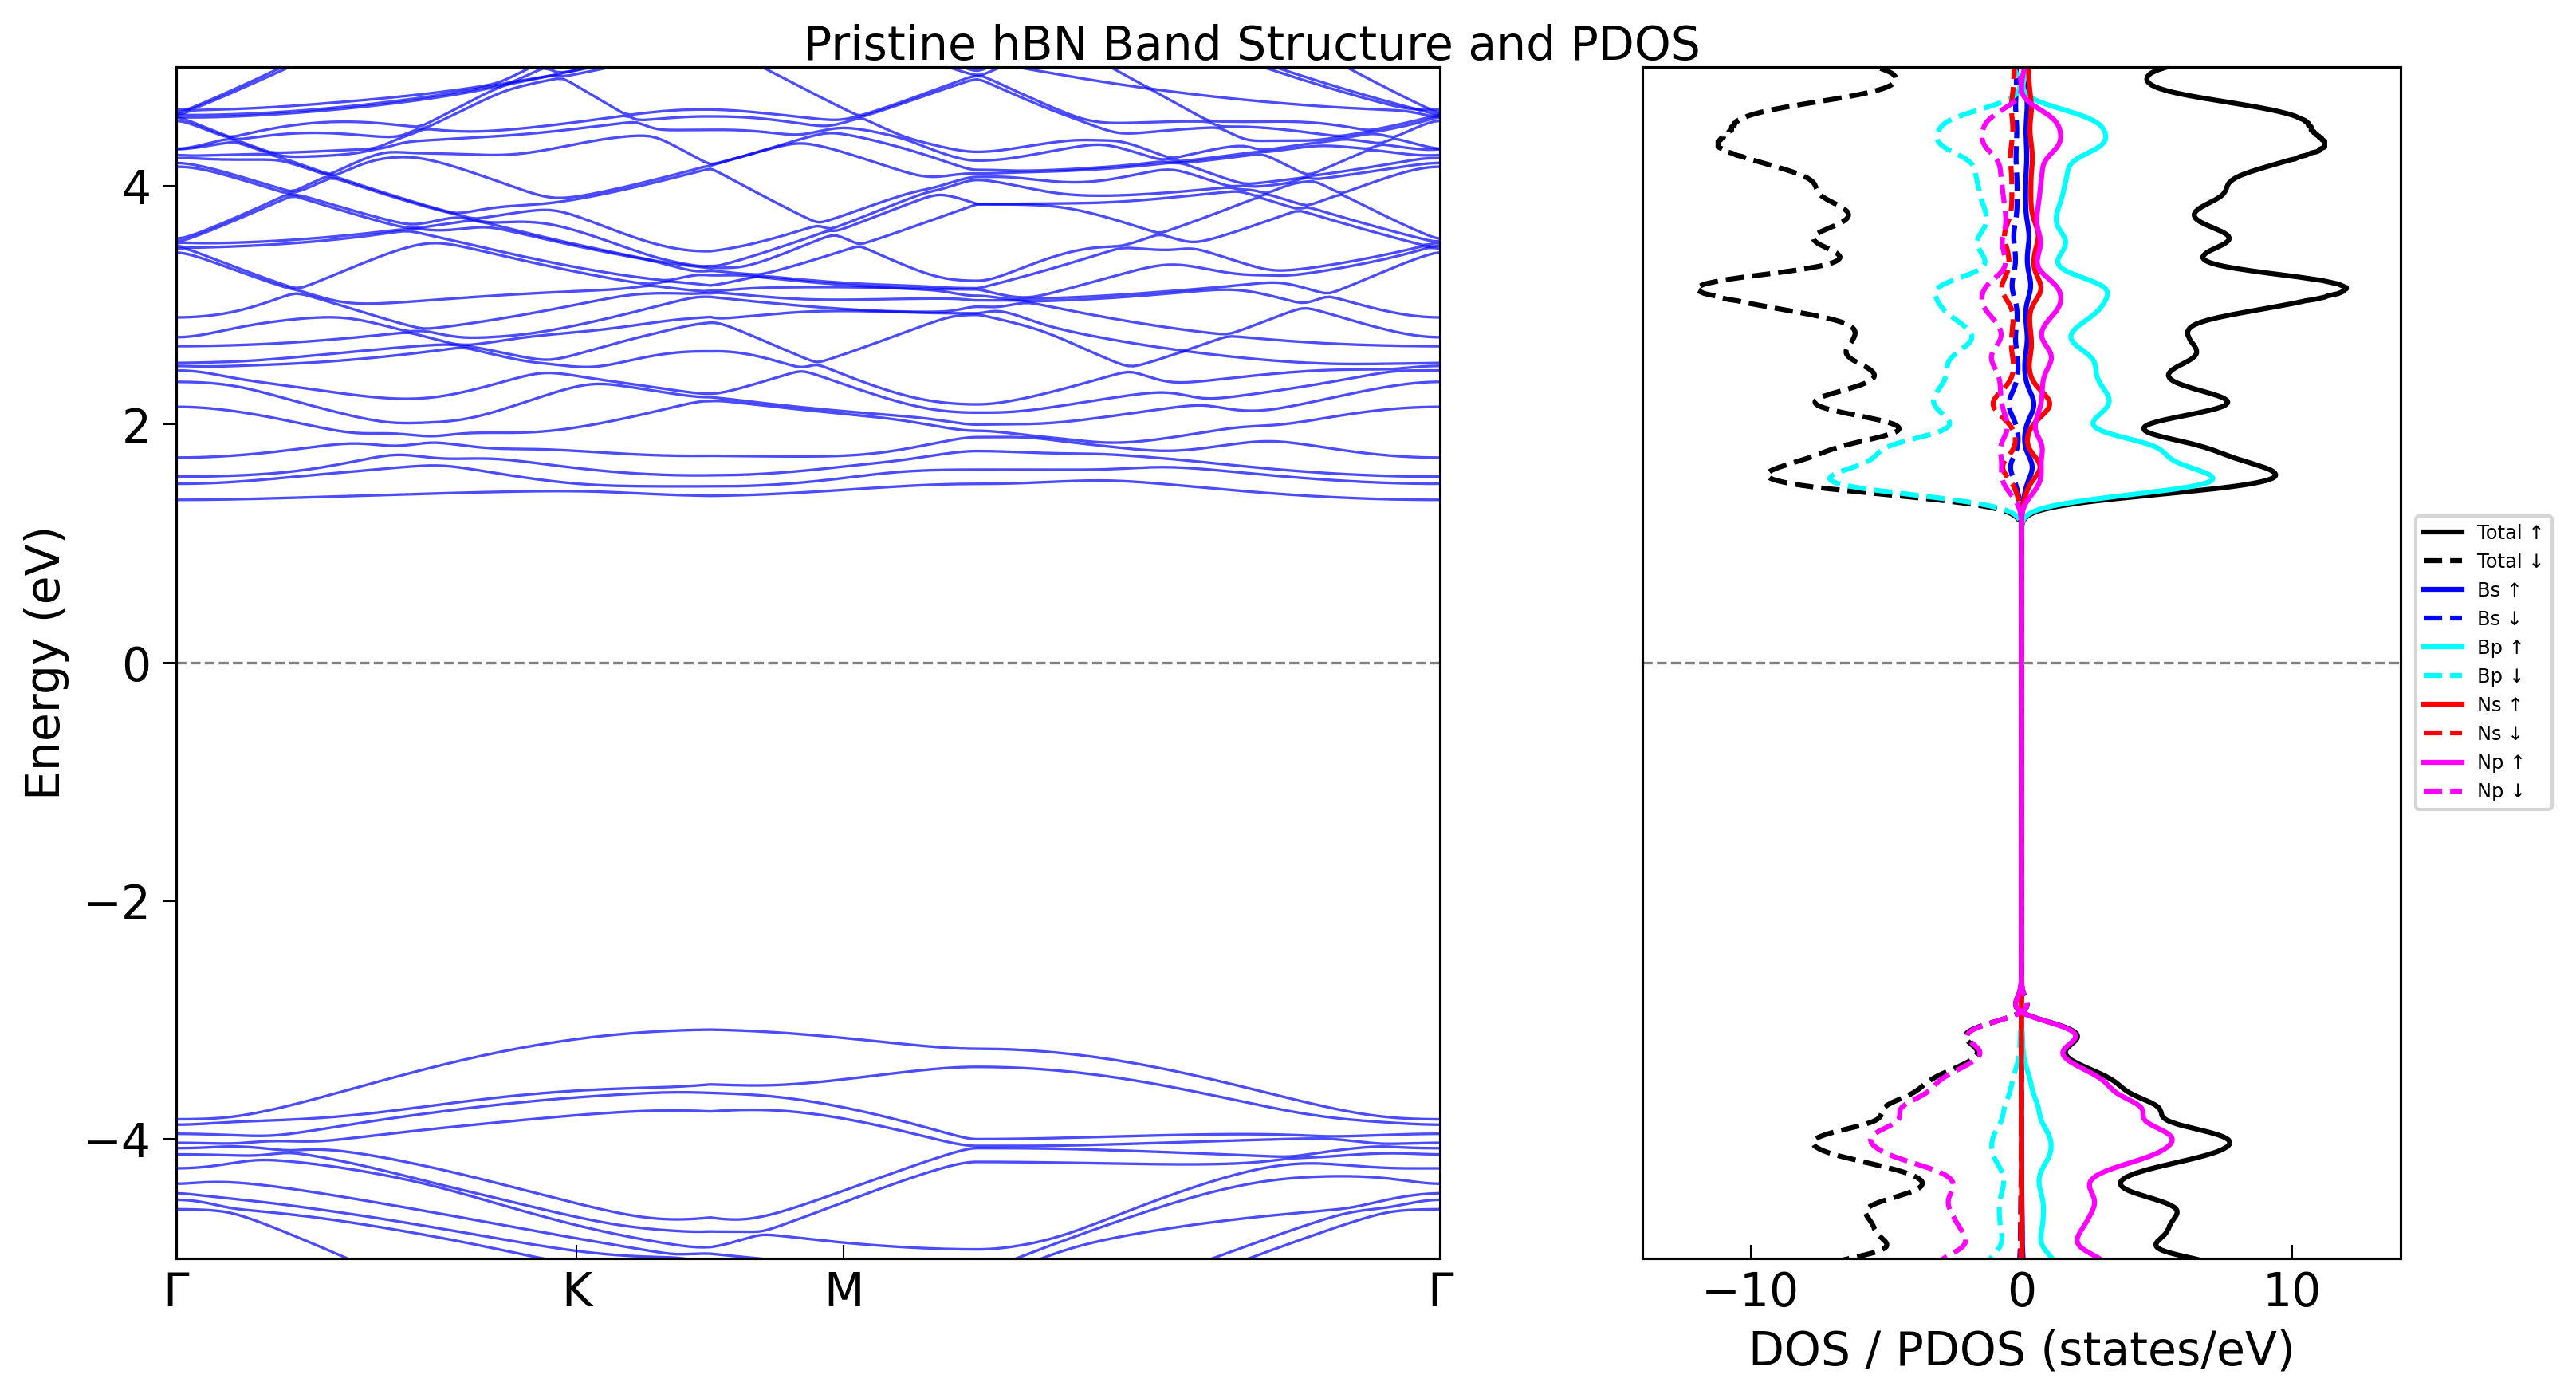
\includegraphics[width=0.9\textwidth]{gambar_hasil/simple_bands_pdos_pristine.png}
    \caption{Struktur pita elektronik dan Kerapatan Keadaan Terproyeksi (PDOS) untuk monolayer hBN murni (\textit{pristine}). Energi Fermi diset sebagai referensi energi nol pada plot PDOS.}
    \label{fig:hbn_pristine_bs_pdos}
\end{figure}

Analisis kerapatan muatan elektronik 3D untuk hBN murni menunjukkan akumulasi densitas elektron yang lebih tinggi di sekitar atom nitrogen dibandingkan dengan atom boron. Fenomena ini konsisten dengan perbedaan elektronegativitas antara nitrogen dan boron, di mana nitrogen lebih elektronegatif. Akibatnya, ikatan B-N dalam hBN bersifat kovalen polar, dengan transfer muatan parsial dari boron ke nitrogen . 
\begin{figure}[h!]
    \centering
    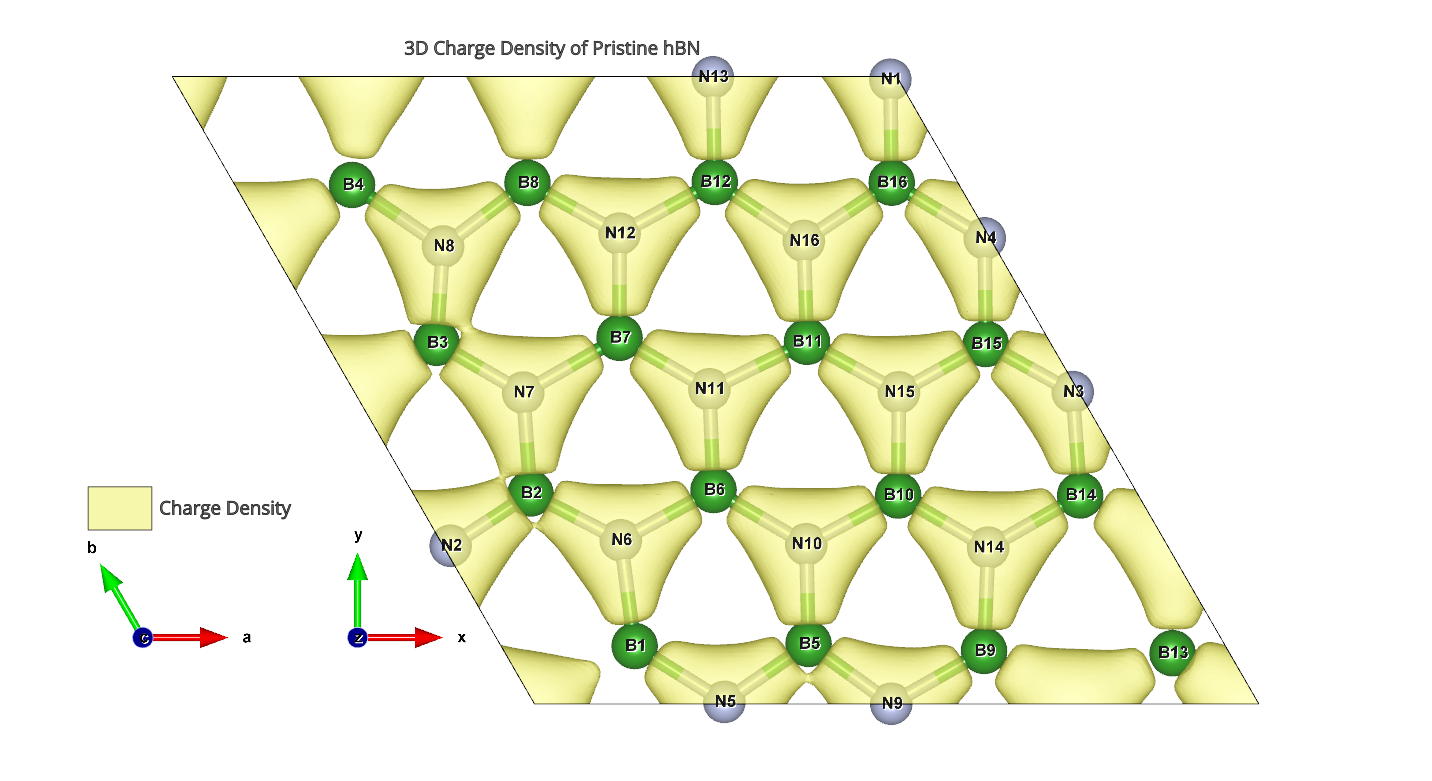
\includegraphics[width=0.9\textwidth]{gambar_hasil/hBN_rho_3d_pristine.png}
    \caption{Visualisasi kerapatan muatan elektronik 3D untuk monolayer hBN murni (\textit{pristine}). Warna menunjukkan isosurface dari kerapatan muatan.}
    \label{fig:hbn_pristine_chargedensity}
\end{figure}

Nilai celah pita energi sebesar $4.446$ eV yang diperoleh dari kalkulasi PBEsol ini, sebagaimana telah disinggung pada Sub-bab \ref{subsec:dft_qe}, menunjukkan underestimasi yang tipikal untuk fungsional GGA bila dibandingkan dengan nilai eksperimental hBN atau hasil dari metode komputasi yang lebih akurat seperti fungsional hibrid atau GW.Tabel \ref{tab:hbn_murni_literatur} menyajikan perbandingan sifat elektronik hBN murni dari hasil penelitian ini dengan nilai-nilai literatur, yang berfungsi untuk memvalidasi konsistensi hasil PBEsol yang diperoleh dan menetapkan konteks untuk interpretasi perubahan akibat perlakuan termal dan defek. 
\begin{table}[h!]
  \centering
  \caption{Perbandingan Sifat Elektronik Monolayer hBN Murni Hasil Perhitungan dengan Nilai Literatur.}
  \label{tab:hbn_murni_literatur_updated}
  \begin{threeparttable}
    \begin{tabular}{lcccc}
      \toprule
      Properti & Nilai Terhitung & Literatur & Literatur & Eksperimental \\
               & (Penelitian Ini) & PBE (eV)   & Hibrid/GW (eV) & (eV)         \\
      \midrule
      VBM (eV)  & -3.081          & $\sim -3.8$\tnote{a}      & $\sim -4.5$ hingga $-4.2$ & – \\
      CBM (eV)  & 1.365           & $\sim 0.8$\tnote{a}       & $\sim 1.6$ hingga $1.9$   & – \\
      $E_g$ (eV)& 4.446           & $4.66$–$4.74$             & $\sim 5.8$–$7.1$          & $\sim 5.9$–$6.1$ \\
      $E_F$ (eV)& -0.445          & Bervariasi\tnote{b}       & Bervariasi\tnote{b}       & Bervariasi\tnote{b} \\
      \bottomrule
    \end{tabular}
    \begin{tablenotes}[flushleft]
      \footnotesize
      \item[a] Nilai absolut VBM dan CBM sangat bergantung pada penyelarasan level vakum dan dapat bervariasi antar studi. Nilai yang ditampilkan berasal dari \citep{liu2024}.
      \item[b] Tingkat Fermi ($E_F$) berada di tengah celah pita untuk sistem murni (intrinsik), namun nilai absolutnya bergantung pada referensi energi (misalnya, level vakum).
      \item Sumber literatur: PBE/PBEsol: \citep{liu2024,korkmaz2020}; Hibrid/GW: \citep{arnaud2006}; Eksperimental: \citep{Watanabe2004}.
    \end{tablenotes}
  \end{threeparttable}
\end{table}

Perbandingan ini mengonfirmasi bahwa metodologi DFT yang digunakan dalam penelitian ini menghasilkan parameter elektronik dasar untuk hBN murni yang sejalan dengan ekspektasi untuk fungsional PBEsol, termasuk underestimasi celah pita yang diketahui. Hal ini memberikan dasar yang valid untuk menganalisis perubahan relatif pada sifat elektronik akibat perlakuan termal dan introduksi defek.

\subsection{Pengaruh Perlakuan Termal pada hBN Murni (800K, 1100K, dan 1225K)}
\label{subsec:hbn_murni_termal}
Untuk menginvestigasi pengaruh temperatur terhadap sifat elektronik monolayer hBN murni, struktur atomik yang telah direlaksasi melalui simulasi MD pada temperatur 800K, 1100K, dan 1225K digunakan sebagai input untuk kalkulasi DFT. Hasil perhitungan parameter elektronik utama dirangkum dalam Tabel \ref{tab:hbn_murni_suhu} dan diilustrasikan melalui struktur pita serta PDOS pada Gambar \ref{fig:hbn_pure_800K}, \ref{fig:hbn_pure_1100K}, dan \ref{fig:hbn_pure_1225K}. Teramati tren yang konsisten bahwa celah pita energi ($E_g$) monolayer hBN murni menurun seiring dengan meningkatnya temperatur. Nilai $E_g$ berkurang dari $4.446$ eV pada kondisi \textit{pristine} menjadi $4.415$ eV pada 800K, kemudian menjadi $4.328$ eV pada 1100K, dan akhirnya $4.069$ eV pada 1225K.Total reduksi celah pita dari kondisi \textit{pristine} hingga 1225K adalah sekitar $0.377$ eV . Penurunan celah pita ini terutama disebabkan oleh pergeseran CBM ke tingkat energi yang lebih rendah (kurang positif), sementara VBM menunjukkan pergeseran yang lebih kecil dan bervariasi (cenderung ke energi yang lebih rendah atau lebih negatif pada 800K dan 1100K, kemudian sedikit naik pada 1225K namun tetap lebih rendah dari nilai \textit{pristine}) . Energi Fermi ($E_F$) menunjukkan fluktuasi kecil namun secara umum tetap berada di dalam celah pita, mengindikasikan bahwa material tetap bersifat isolator/semikonduktor. Sesuai ekspektasi, sistem hBN murni tetap non-magnetik pada semua temperatur yang diuji, dengan magnetisasi total dan absolut mendekati nol. 
\begin{table}[h!]
  \centering
  \caption{Sifat Elektronik Monolayer hBN Murni sebagai Fungsi Temperatur.}
  \label{tab:hbn_murni_suhu}
  \begin{tabular}{lccccc}
    \toprule
    Temperatur (K) & VBM (eV) & CBM (eV) & $E_g$ (eV) & $\Delta E_g$ dari Pristine (eV) & $E_F$ (eV) \\
    \midrule
    Pristine (Ref.) & -3.081 &  1.365 & 4.446 &  0.000 & -0.445 \\
    800             & -3.238 &  1.177 & 4.415 & -0.031 & -0.304 \\
    1100   
          & -3.183 &  1.145 & 4.328 & -0.118 & -0.323 \\
    1225            & -3.112 &  0.957 & 4.069 & -0.377 & -0.430 \\
    \bottomrule
  \end{tabular}
\end{table}

\begin{figure}[h!]
    \centering
    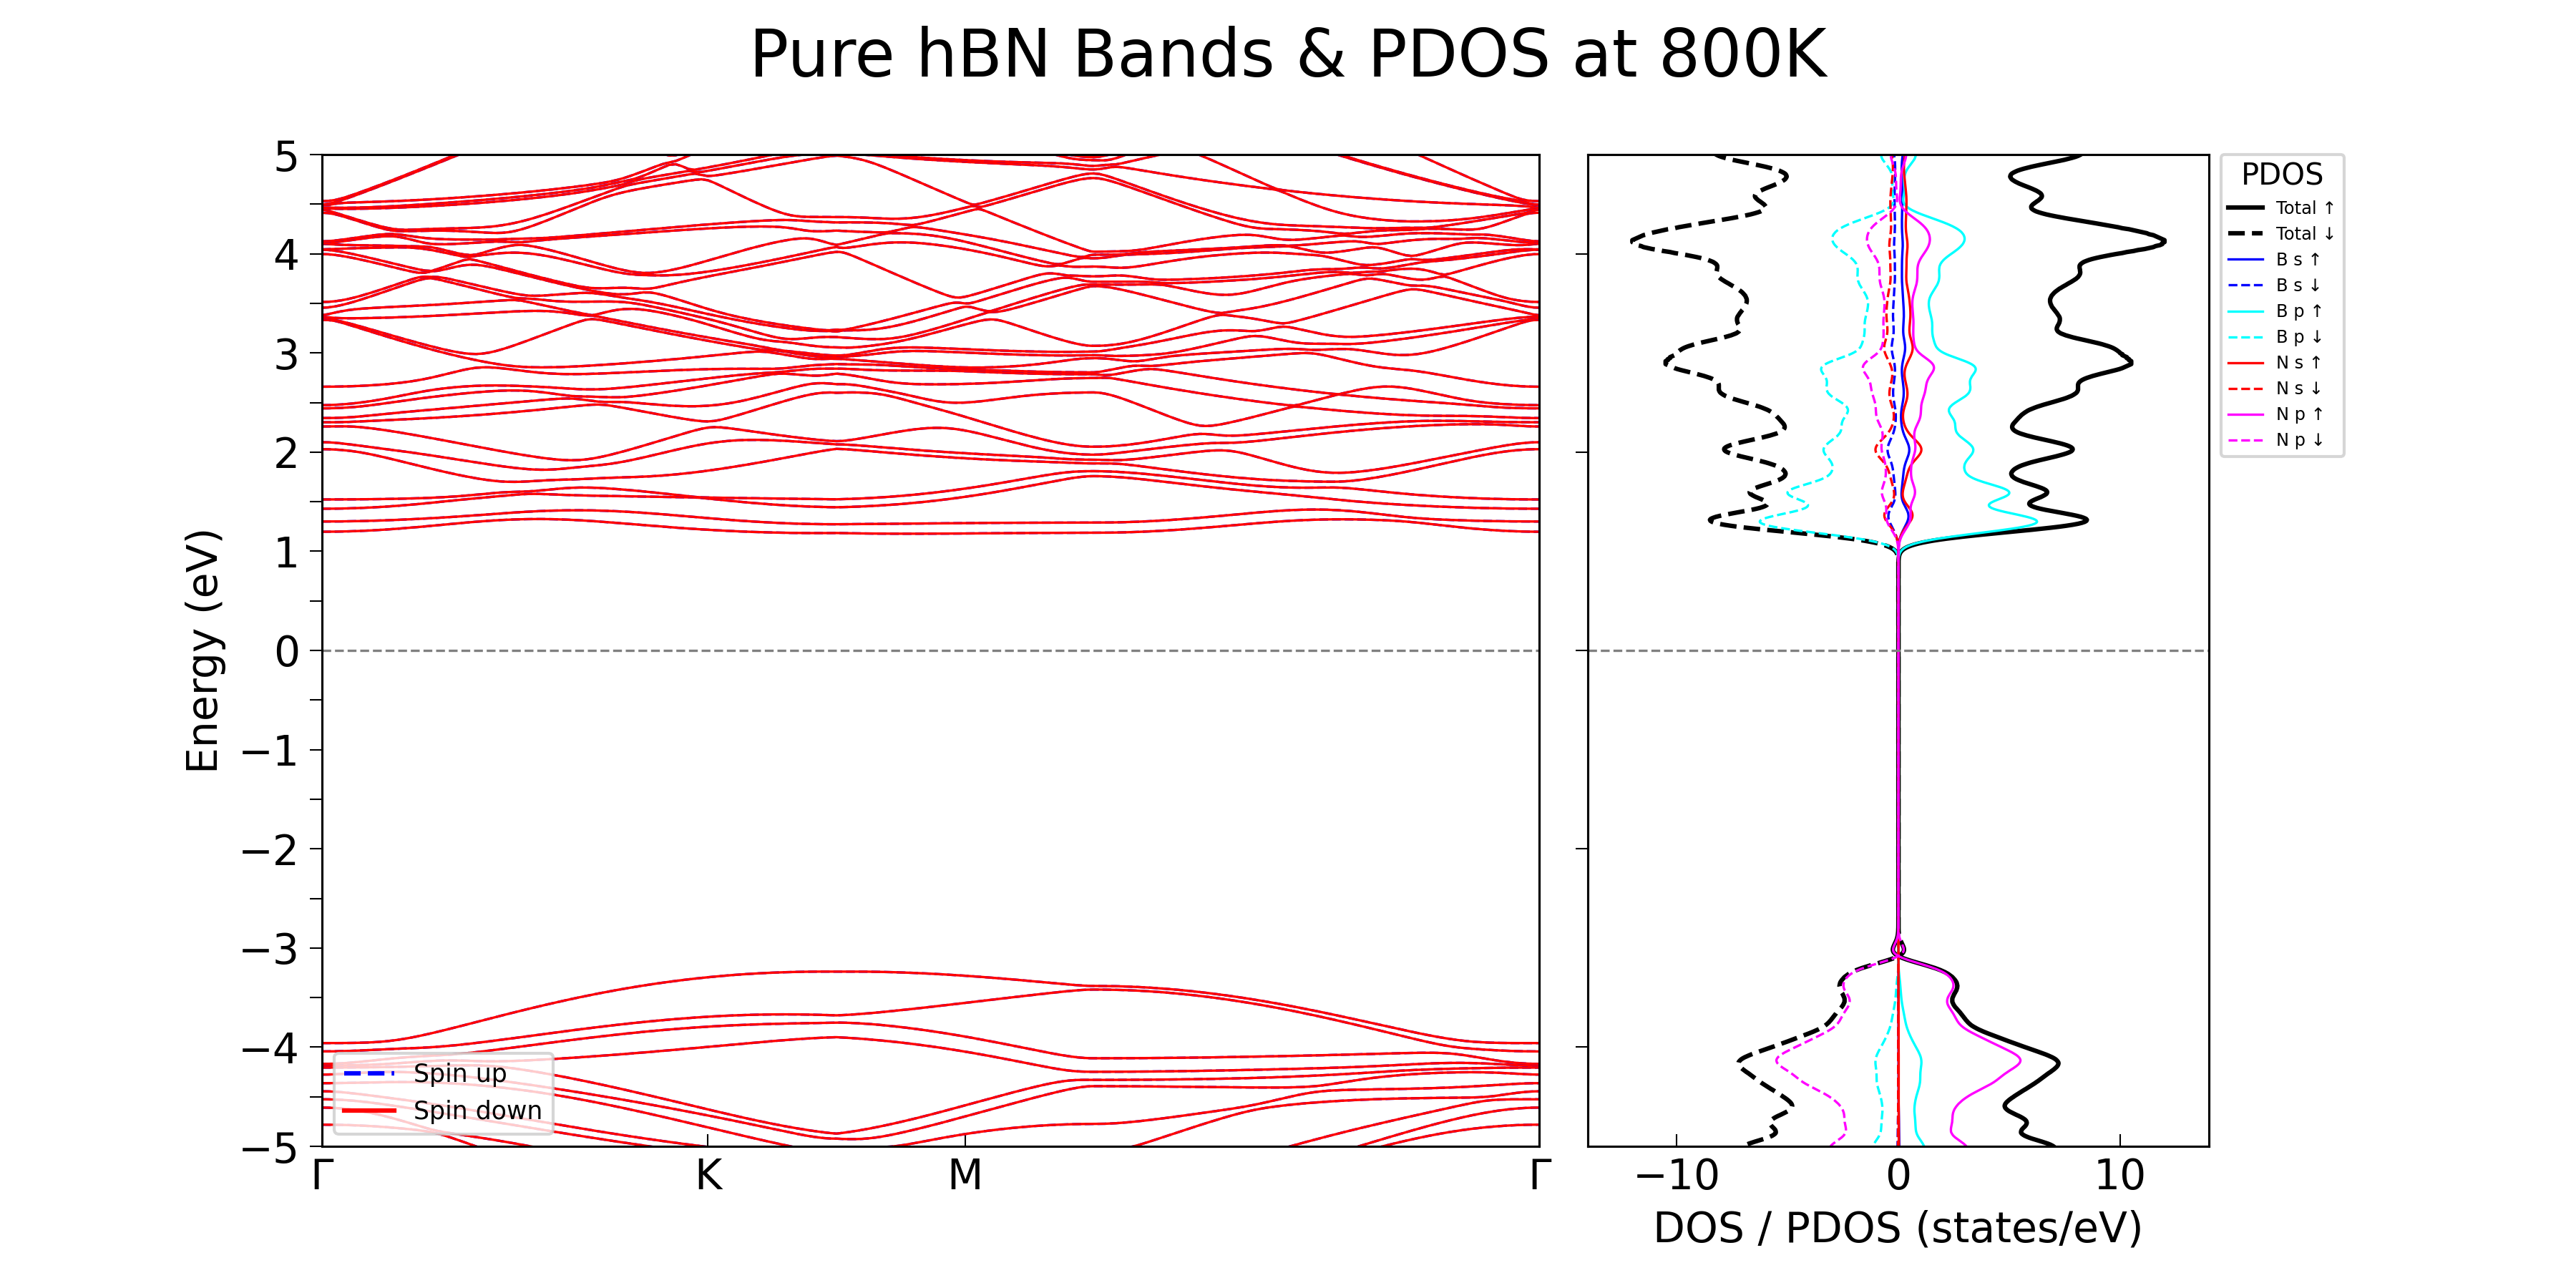
\includegraphics[width=0.9\textwidth]{gambar_hasil/simple_bands_pdos_pure_800K.png}
    \caption{Struktur pita elektronik dan PDOS untuk monolayer hBN murni pada 800K. [1]}
    \label{fig:hbn_pure_800K}
\end{figure}

\begin{figure}[h!]
    \centering
    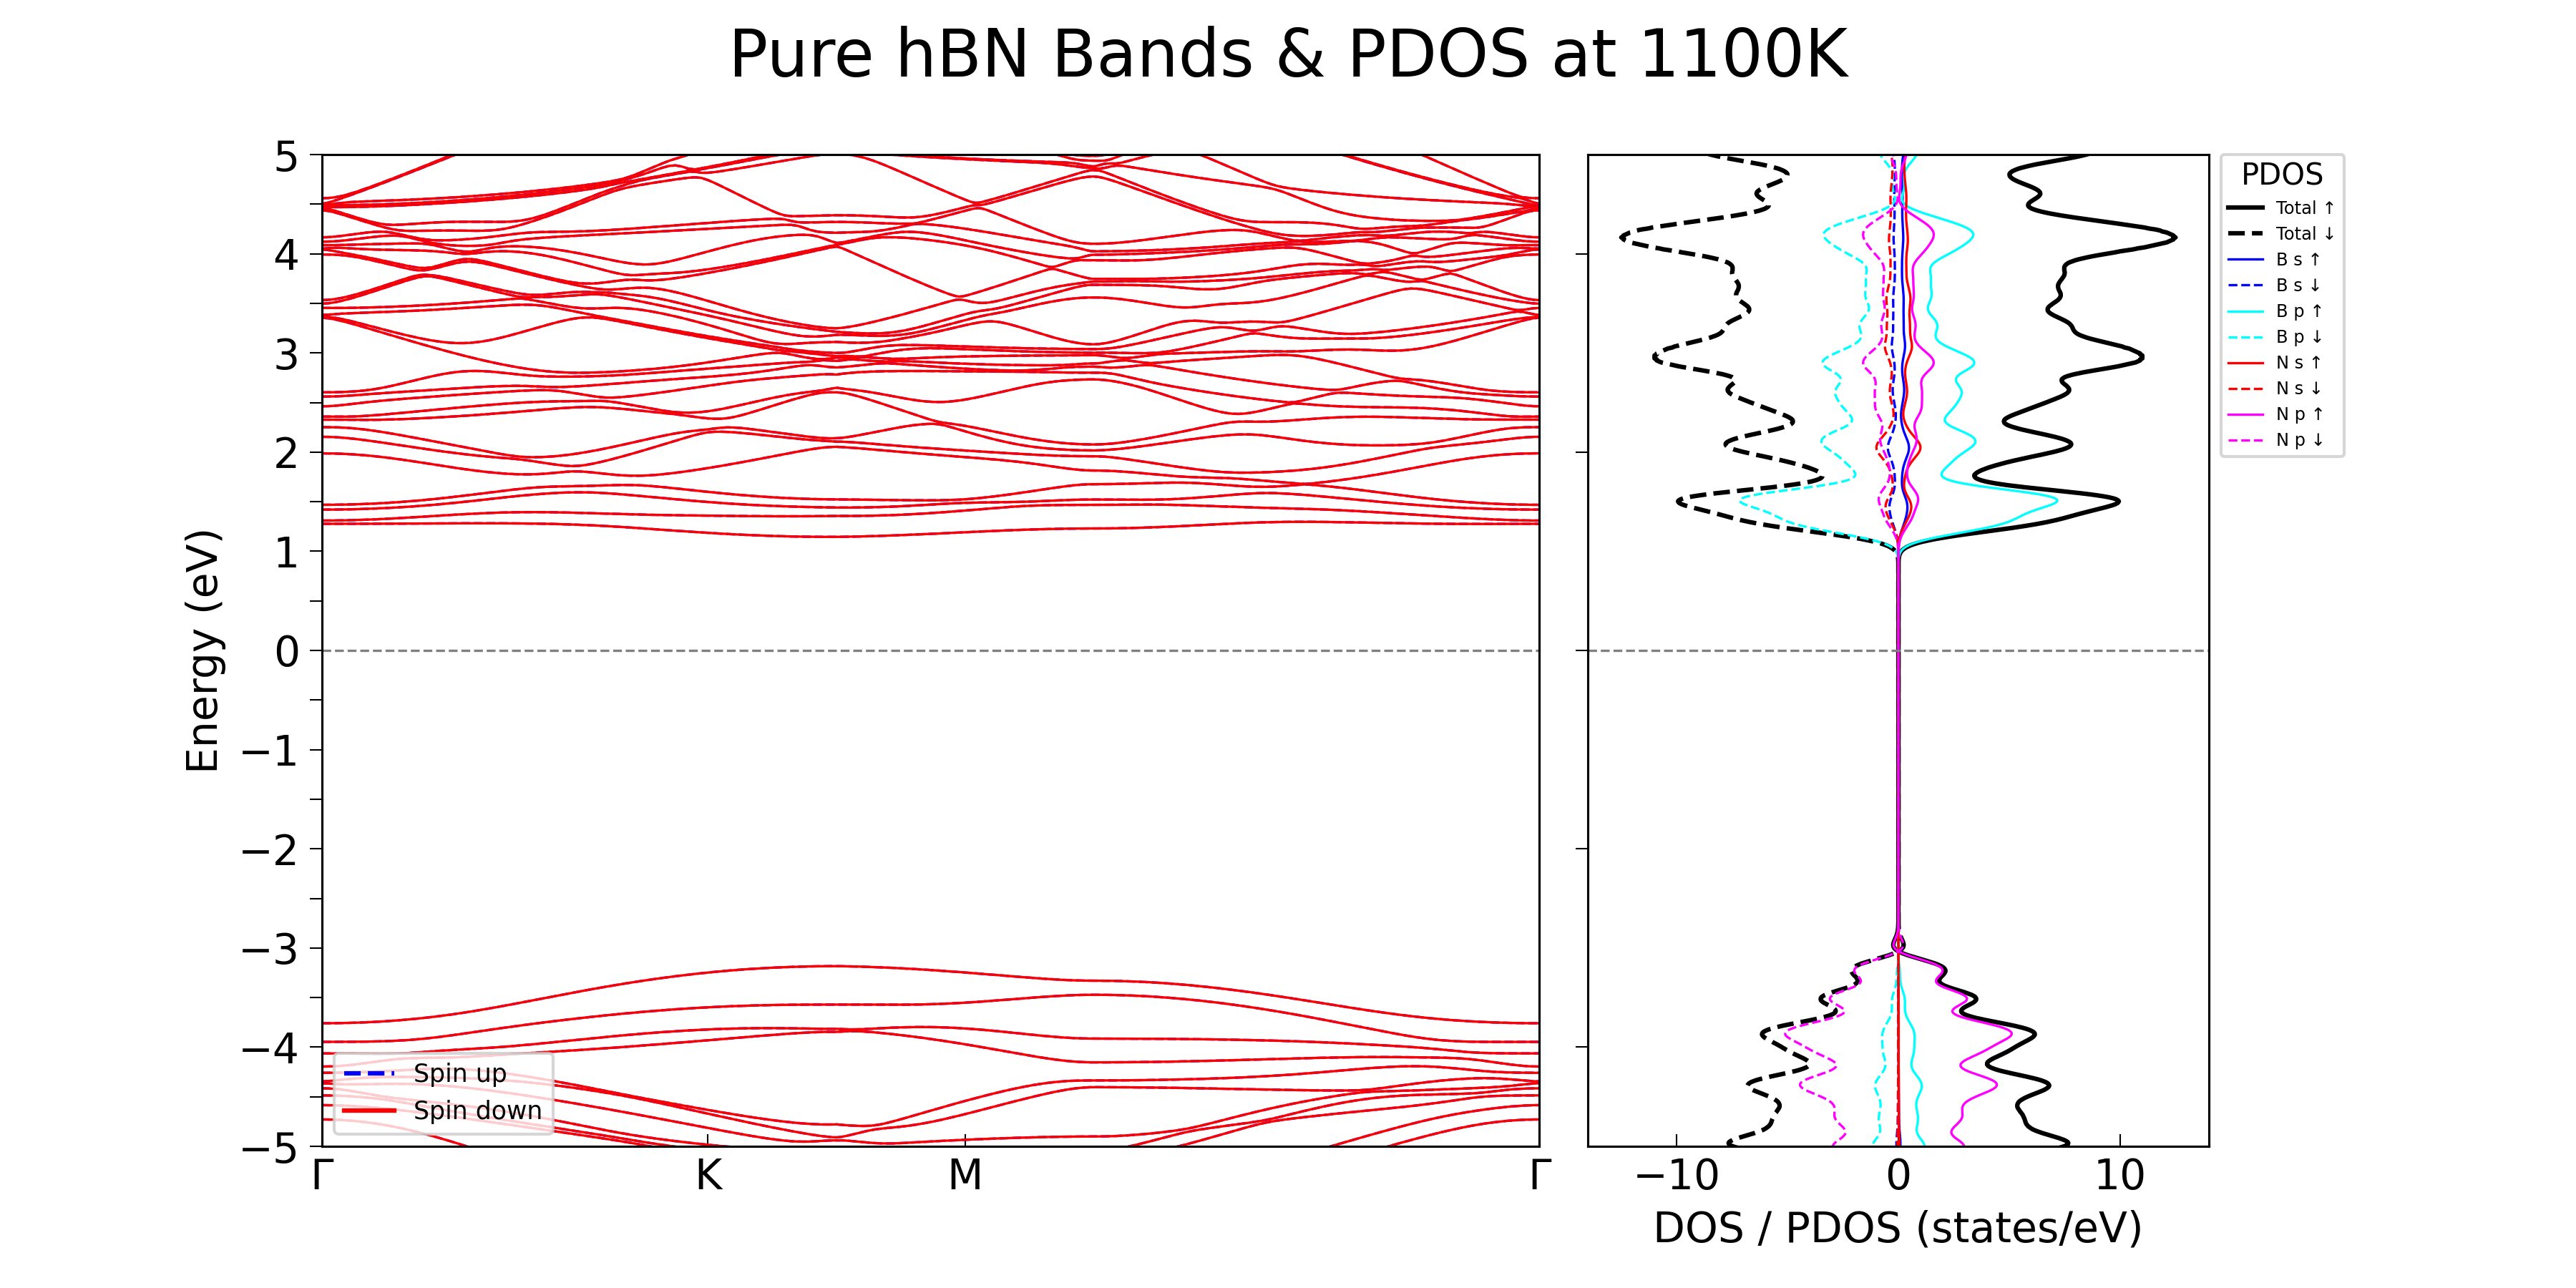
\includegraphics[width=0.9\textwidth]{gambar_hasil/simple_bands_pdos_pure_1100K.png}
    \caption{Struktur pita elektronik dan PDOS untuk monolayer hBN murni pada 1100K. [1]}
    \label{fig:hbn_pure_1100K}
\end{figure}

\begin{figure}[h!]
    \centering
    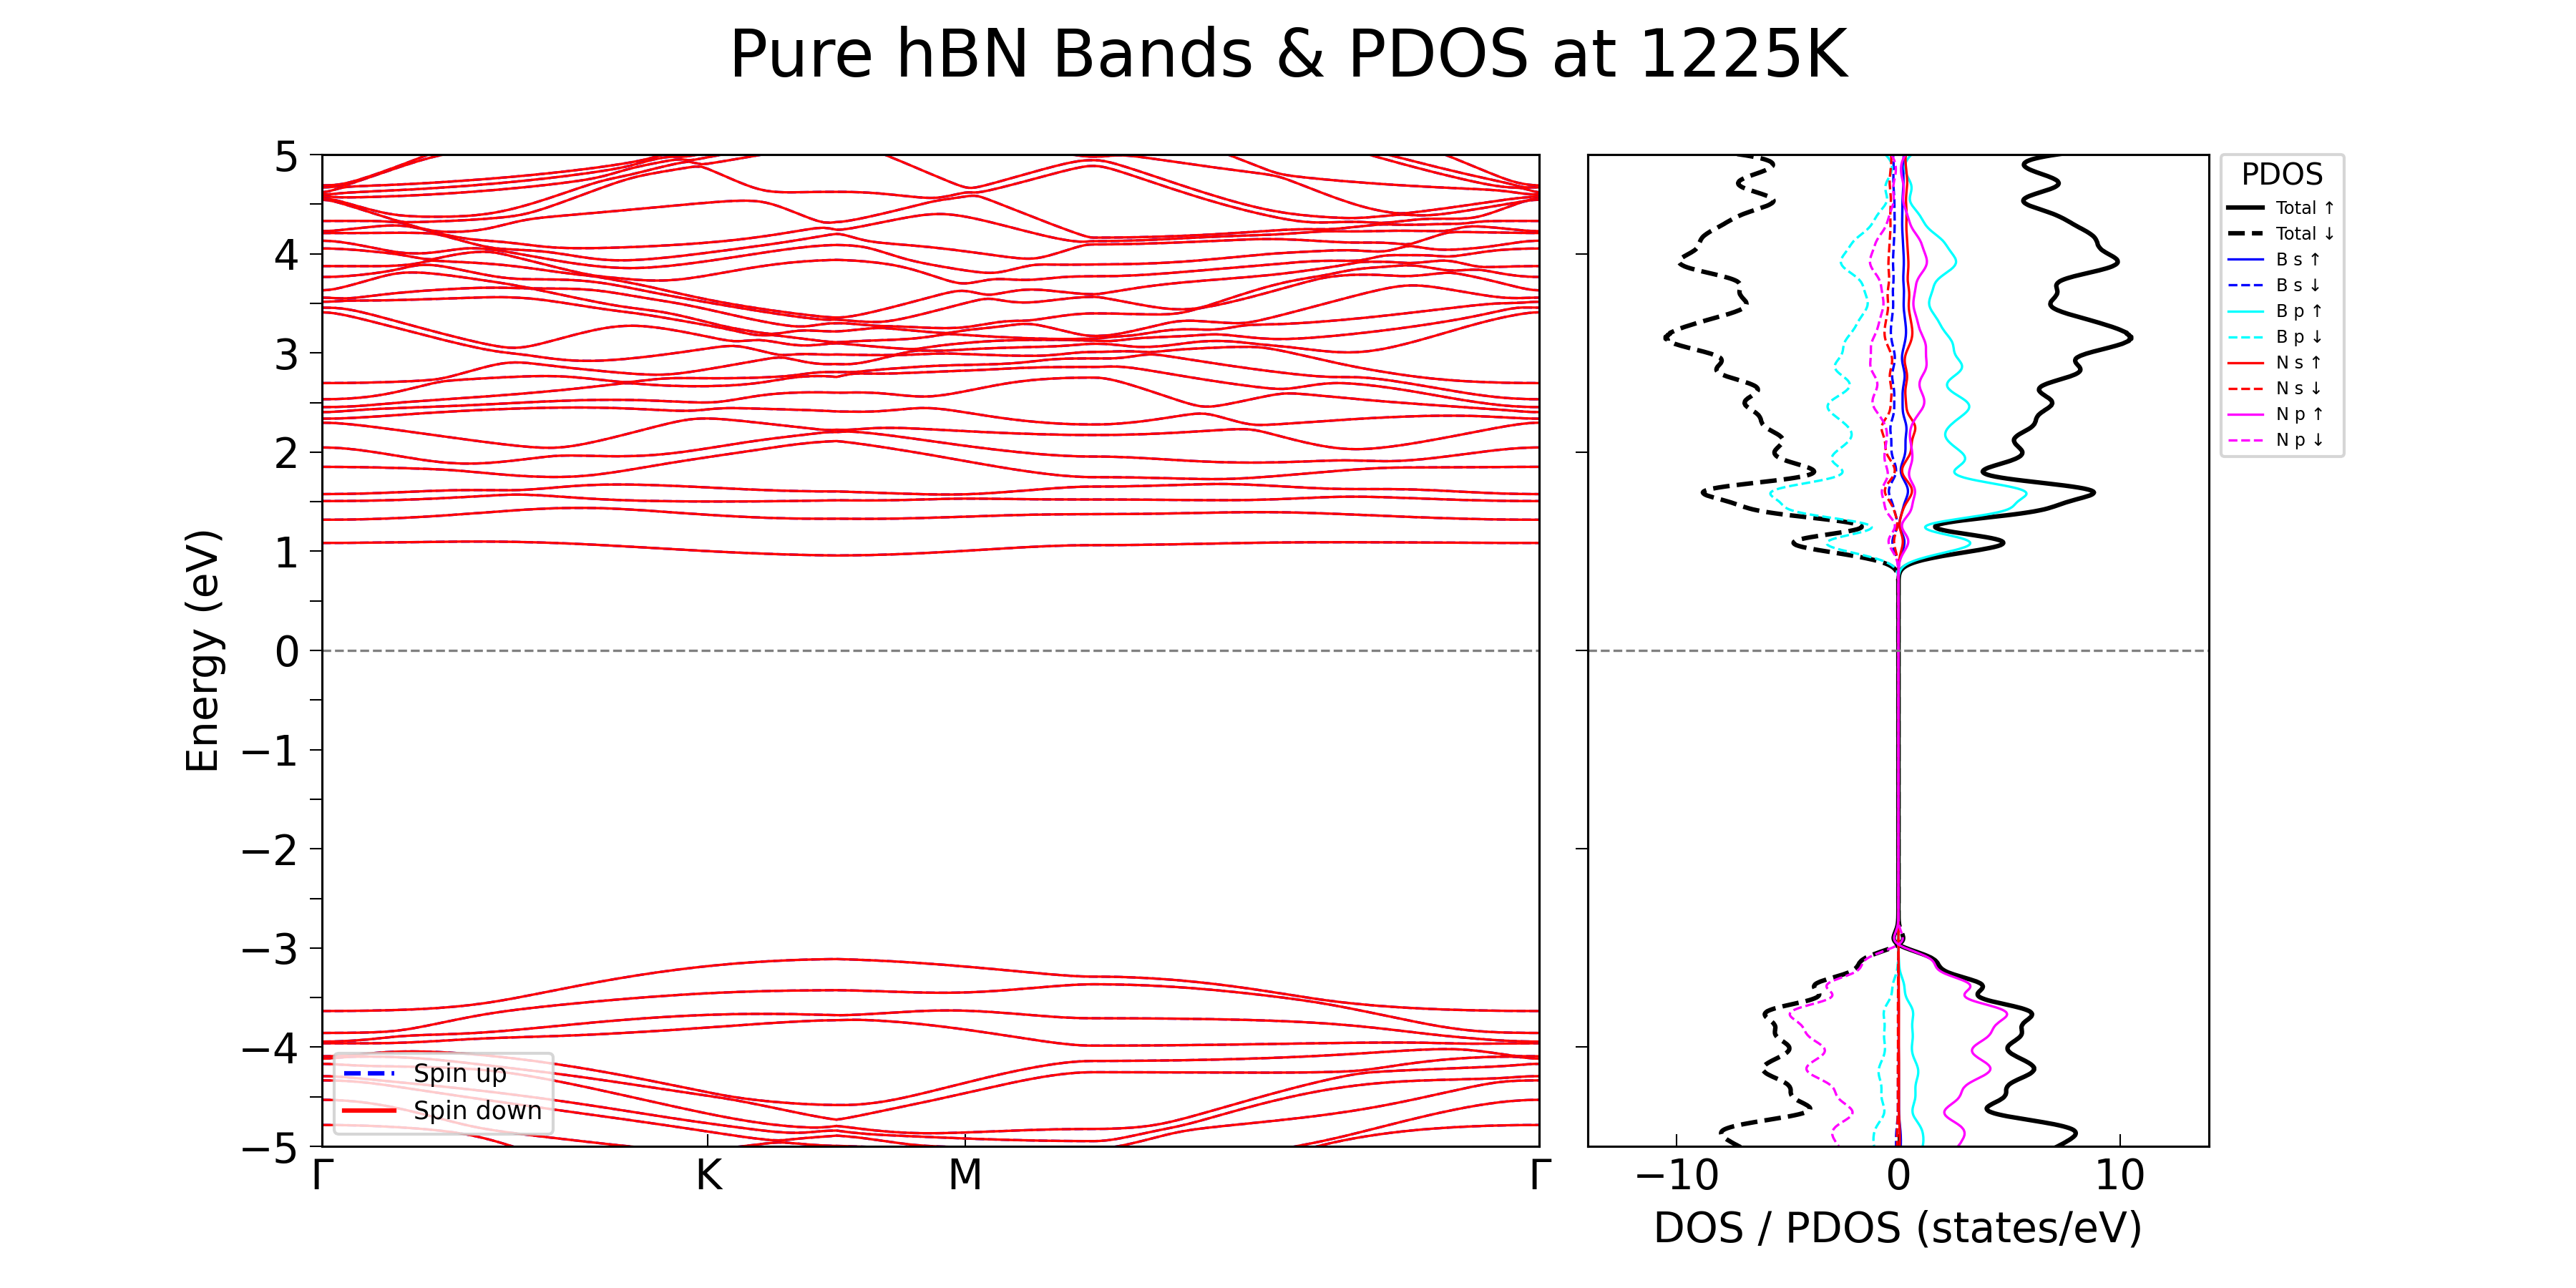
\includegraphics[width=0.9\textwidth]{gambar_hasil/simple_bands_pdos_pure_1225K.png}
    \caption{Struktur pita elektronik dan PDOS untuk monolayer hBN murni pada 1225K. [1]}
    \label{fig:hbn_pure_1225K}
\end{figure}

Penurunan celah pita energi dengan meningkatnya temperatur merupakan fenomena yang umum diamati pada sebagian besar material semikonduktor dan isolator. Fenomena ini dapat diatribusikan pada dua mekanisme utama yang berkontribusi secara simultan: kopling elektron-fonon (\textit{electron-phonon coupling}, EPC) dan ekspansi termal kisi \citep{prethesis2}. Peningkatan temperatur menyebabkan atom-atom dalam kisi bergetar dengan amplitudo yang lebih besar, meningkatkan populasi fonon. Interaksi antara elektron dan vibrasi kisi (fonon) ini menyebabkan renormalisasi energi pita elektronik, yang umumnya mengarah pada penyempitan celah pita. Kontribusi dari EPC seringkali menjadi efek yang dominan, terutama pada temperatur tinggi . Istilah-istilah teoritis seperti kontribusi Debye-Waller (terkait dengan perpindahan atomik kuadrat rata-rata) dan koreksi energi-diri Fan-Migdal digunakan untuk mendeskripsikan efek EPC ini secara lebih detail . Selain itu, peningkatan temperatur umumnya menyebabkan ekspansi termal pada kisi kristal (meskipun ada pengecualian). Ekspansi ini mengubah jarak antar atom dan tumpang-tindih orbital elektronik, yang juga dapat berkontribusi pada perubahan, biasanya penurunan, celah pita energi . Simulasi MD yang dilakukan untuk menghasilkan struktur pada temperatur target secara implisit telah menyertakan efek ekspansi termal ini, namun akurasinya bergantung pada kualitas potensial ReaxFF yang digunakan dalam menangkap respons termomekanik material. Menariknya, beberapa studi literatur mengenai ketergantungan temperatur celah pita pada hBN multilayer melaporkan perilaku yang lebih kompleks, yaitu pergeseran merah (\textit{redshift}) atau penyempitan celah pita pada temperatur rendah (misalnya, di bawah 100K), yang didominasi oleh interaksi elektron-fonon, diikuti oleh pergeseran biru (\textit{blueshift}) atau pelebaran celah pita pada temperatur yang lebih tinggi (misalnya, di atas 100K hingga sekitar 800K) \citep{prethesis2}. Blueshift anomali pada hBN multilayer ini diatribusikan pada perilaku unik dari koefisien ekspansi termal negatif pada bidang (\textit{in-plane}) hBN dalam rentang temperatur tertentu, di mana kisi justru menyusut dengan kenaikan temperatur. Hasil kalkulasi saat ini untuk monolayer hBN pada rentang temperatur yang lebih tinggi (800K hingga 1225K) secara konsisten menunjukkan penyempitan celah pita (redshift). Perbedaan perilaku termal antara monolayer hBN (dalam penelitian ini) dan hBN multilayer (dalam literatur) menyoroti pentingnya efek dimensionalitas. Pada monolayer, kontribusi dari perubahan parameter kisi akibat temperatur mungkin berbeda, atau efek interaksi elektron-fonon menjadi lebih dominan dibandingkan dengan sistem multilayer, terutama pada rentang temperatur tinggi yang dikaji. Vibrasi atom pada permukaan 2D mungkin memiliki dampak yang lebih langsung dan kuat pada interaksi elektron-fonon. Selain itu, ada kemungkinan bahwa potensial ReaxFF yang digunakan, yang diparameterisasi untuk sintesis nanostruktur fasa gas \citep{Lele2022}, mungkin tidak secara akurat menangkap karakteristik ekspansi termal negatif yang spesifik untuk monolayer hBN, jika memang ada pada rentang temperatur ini. Akibatnya, struktur yang dihasilkan MD mungkin tidak menunjukkan kontraksi kisi yang diperlukan untuk blueshift, dan kalkulasi DFT kemudian akan mencerminkan respons elektronik terhadap konfigurasi atomik tersebut. Dengan demikian, untuk monolayer hBN dalam kondisi temperatur yang dikaji dalam penelitian ini, pelebaran pita energi akibat vibrasi kisi yang meningkat tampaknya menjadi faktor utama yang menentukan penyempitan celah pita yang teramati. 
\section{Dampak Defek Antisite pada Sifat Elektronik dan Magnetik hBN}
\label{sec:hbn_defek}
Kehadiran defek titik dalam kisi kristal dapat secara dramatis mengubah sifat elektronik dan magnetik material, seringkali dengan cara yang tidak terduga dan berpotensi bermanfaat untuk aplikasi tertentu. Bagian ini akan membahas secara rinci pengaruh dua jenis defek antisite, yaitu defek Nitrogen pada situs Boron (N$_B$) dan defek Boron pada situs Nitrogen (B$_N$), terhadap sifat-sifat monolayer hBN pada berbagai temperatur. Berdasarkan hasil kalkulasi, "NN defect" yang disebutkan dalam data hasil kalkulasi  diinterpretasikan sebagai defek antisite N$_B$, di mana sebuah atom Nitrogen menempati situs yang seharusnya diisi oleh atom Boron. Sementara itu, "BB defect" diinterpretasikan sebagai defek antisite B$_N$, di mana sebuah atom Boron menempati situs yang seharusnya diisi oleh atom Nitrogen. 
\subsection{Monolayer hBN dengan Defek Antisite N$_B$ ("NN defect")}
\label{subsec:hbn_defek_nb}
Defek antisite Nitrogen (N$_B$) mengintroduksi perubahan signifikan pada lingkungan kimia dan elektronik lokal di dalam monolayer hBN. Literatur telah mengaitkan defek N$_B$, khususnya dalam keadaan bermuatan positif (N$_B^+$), dengan emisi optik di daerah biru dengan Garis Fonon Nol (\textit{Zero-Phonon Line}, ZPL) sekitar 2.63 eV. Data hasil kalkulasi untuk hBN dengan defek N$_B$ pada temperatur 800K, 1100K, dan 1225K dirangkum dalam Tabel \ref{tab:hbn_defek_nb} dan diilustrasikan pada Gambar \ref{fig:hbn_NN_800K} hingga \ref{fig:hbn_NN_1225K_chargedensity}. 
\begin{table}[h!]
  \centering
  \caption{Sifat Elektronik Monolayer hBN dengan Defek Antisite N$_B$ sebagai Fungsi Temperatur.}
  \label{tab:hbn_defek_nb}
  \begin{tabular}{lcccccc}
    \toprule
    Temperatur & VBM & CBM & $E_g$ & $E_F$ & Magnetisasi & Magnetisasi \\
    (K) & (eV) & (eV) & (eV) & (eV) & Total ($\mu_B$) & Absolut ($\mu_B$) \\
    \midrule
    800  & -0.448 &  0.246 & 0.694 & -2.538 & 0.000 & 0.000 \\
    1100 & -0.666 &  0.423 & 1.089 & -2.682 &  0.000 & 0.000 
 \\
    1225 & -0.732 &  0.482 & 1.214 & -2.237 & -0.000 & 0.010 \\
    \bottomrule
  \end{tabular}
\end{table}

\begin{figure}[h!]
    \centering
    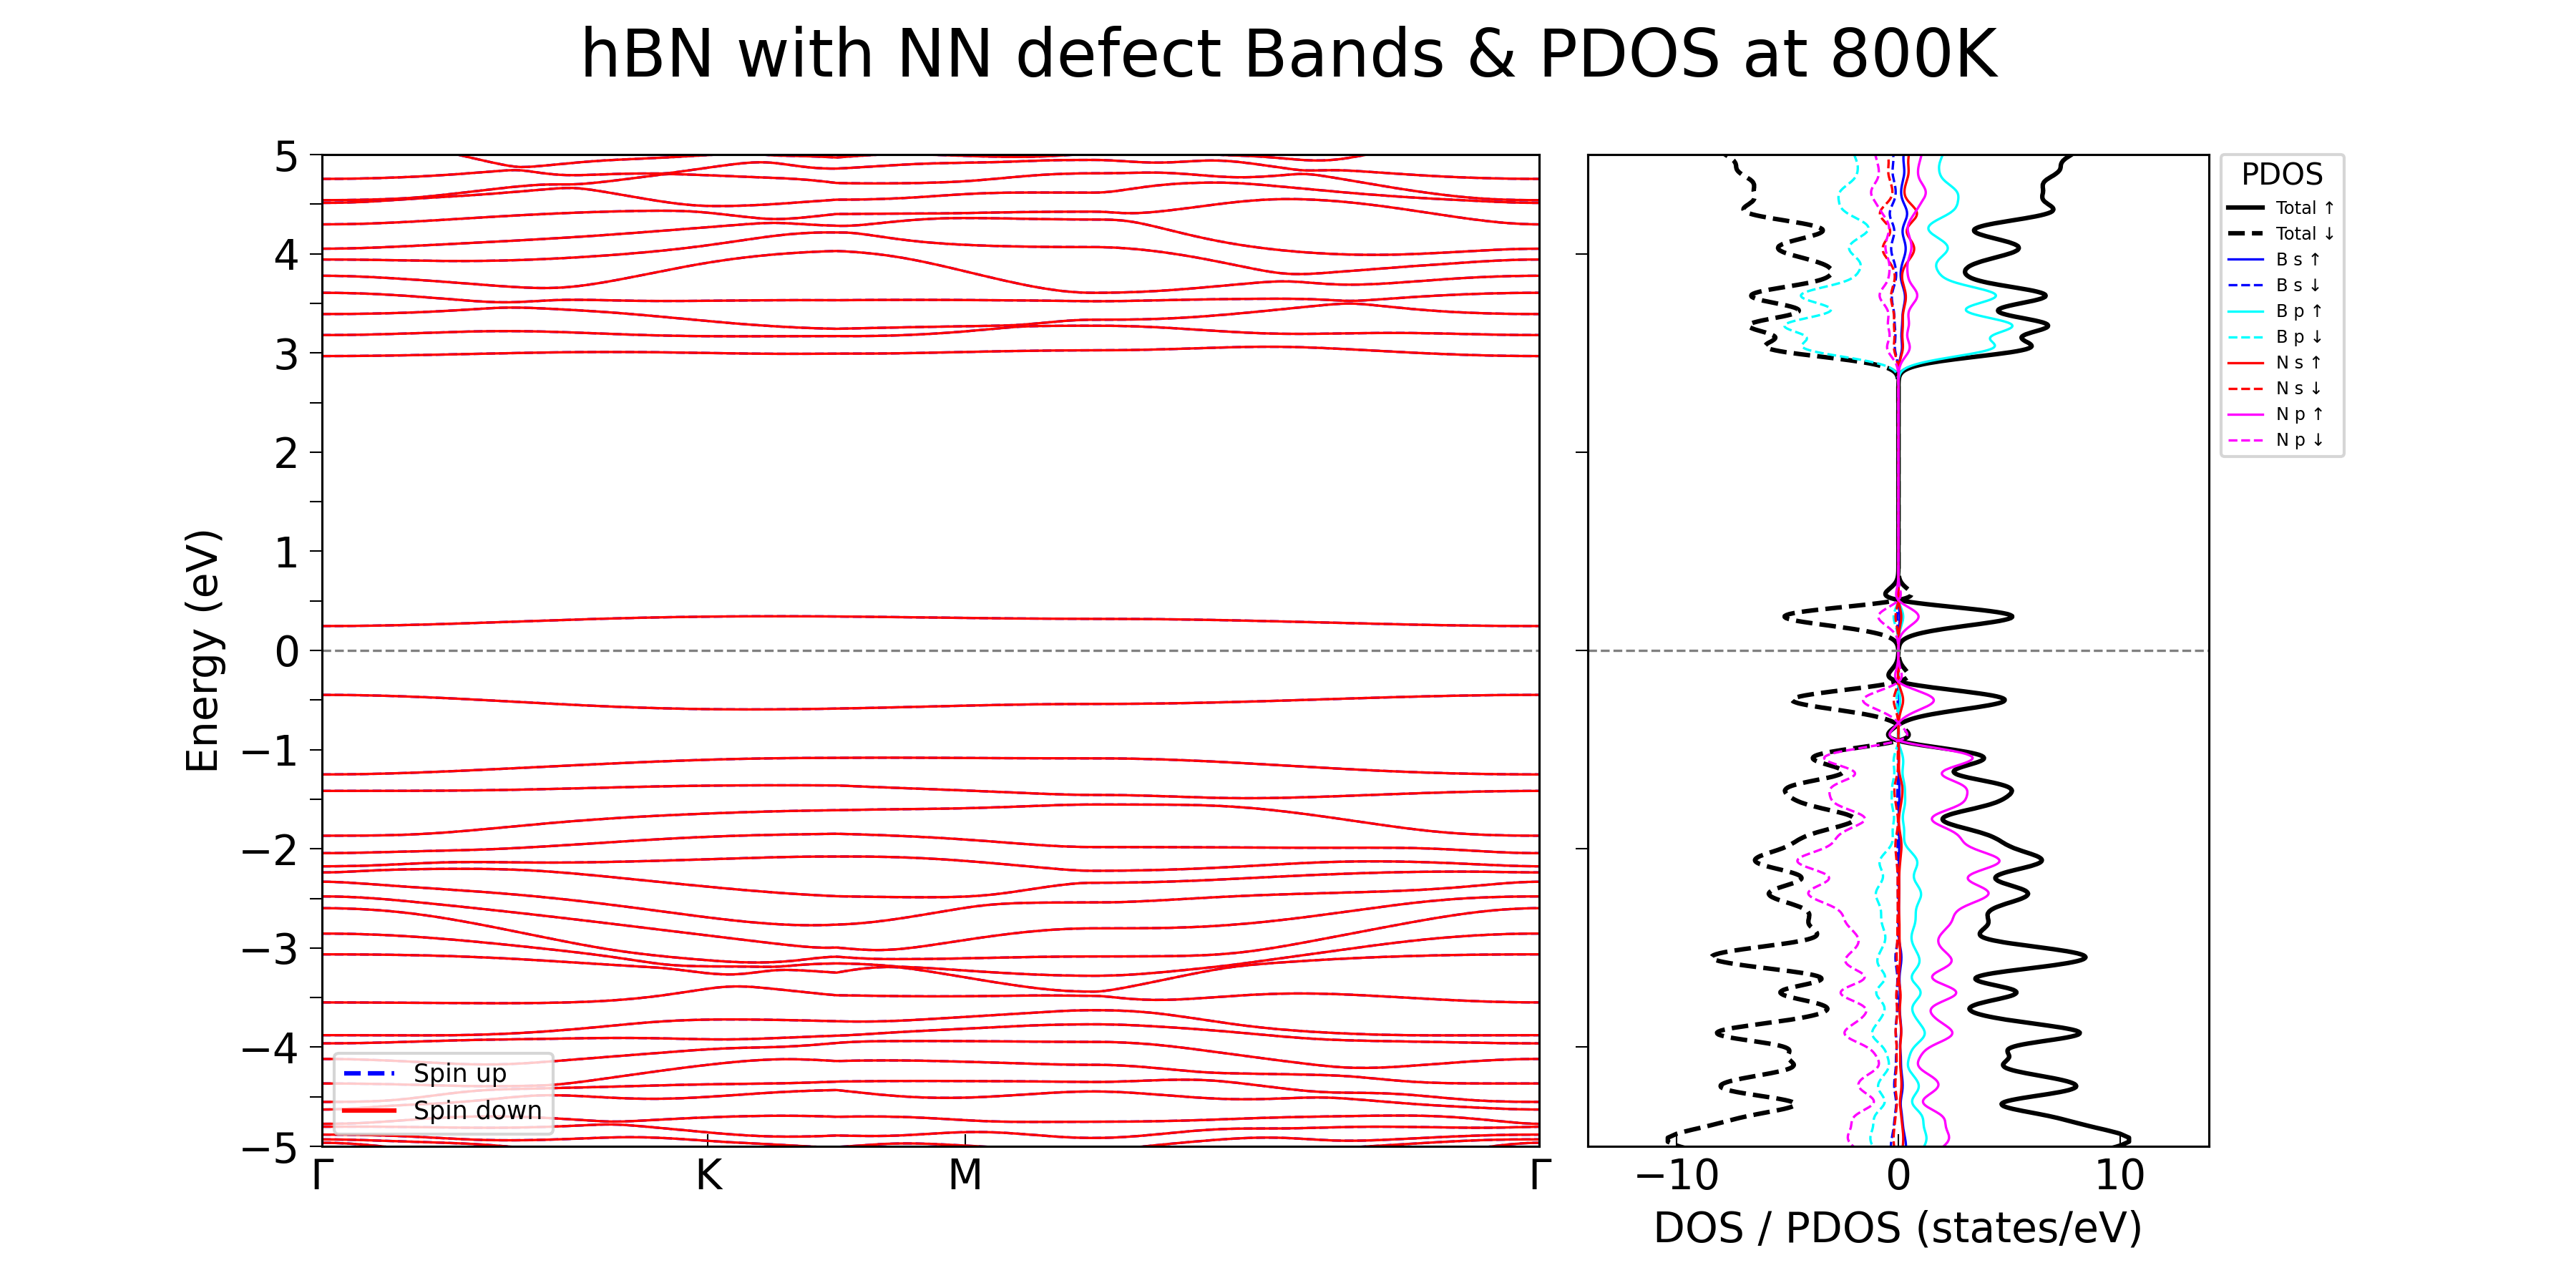
\includegraphics[width=0.9\textwidth]{gambar_hasil/simple_bands_pdos_NN_800K.png}
    \caption{Struktur pita elektronik dan PDOS untuk monolayer hBN dengan defek N$_B$ pada 800K.}
    \label{fig:hbn_NN_800K}
\end{figure}
\begin{figure}[h!]
    \centering
    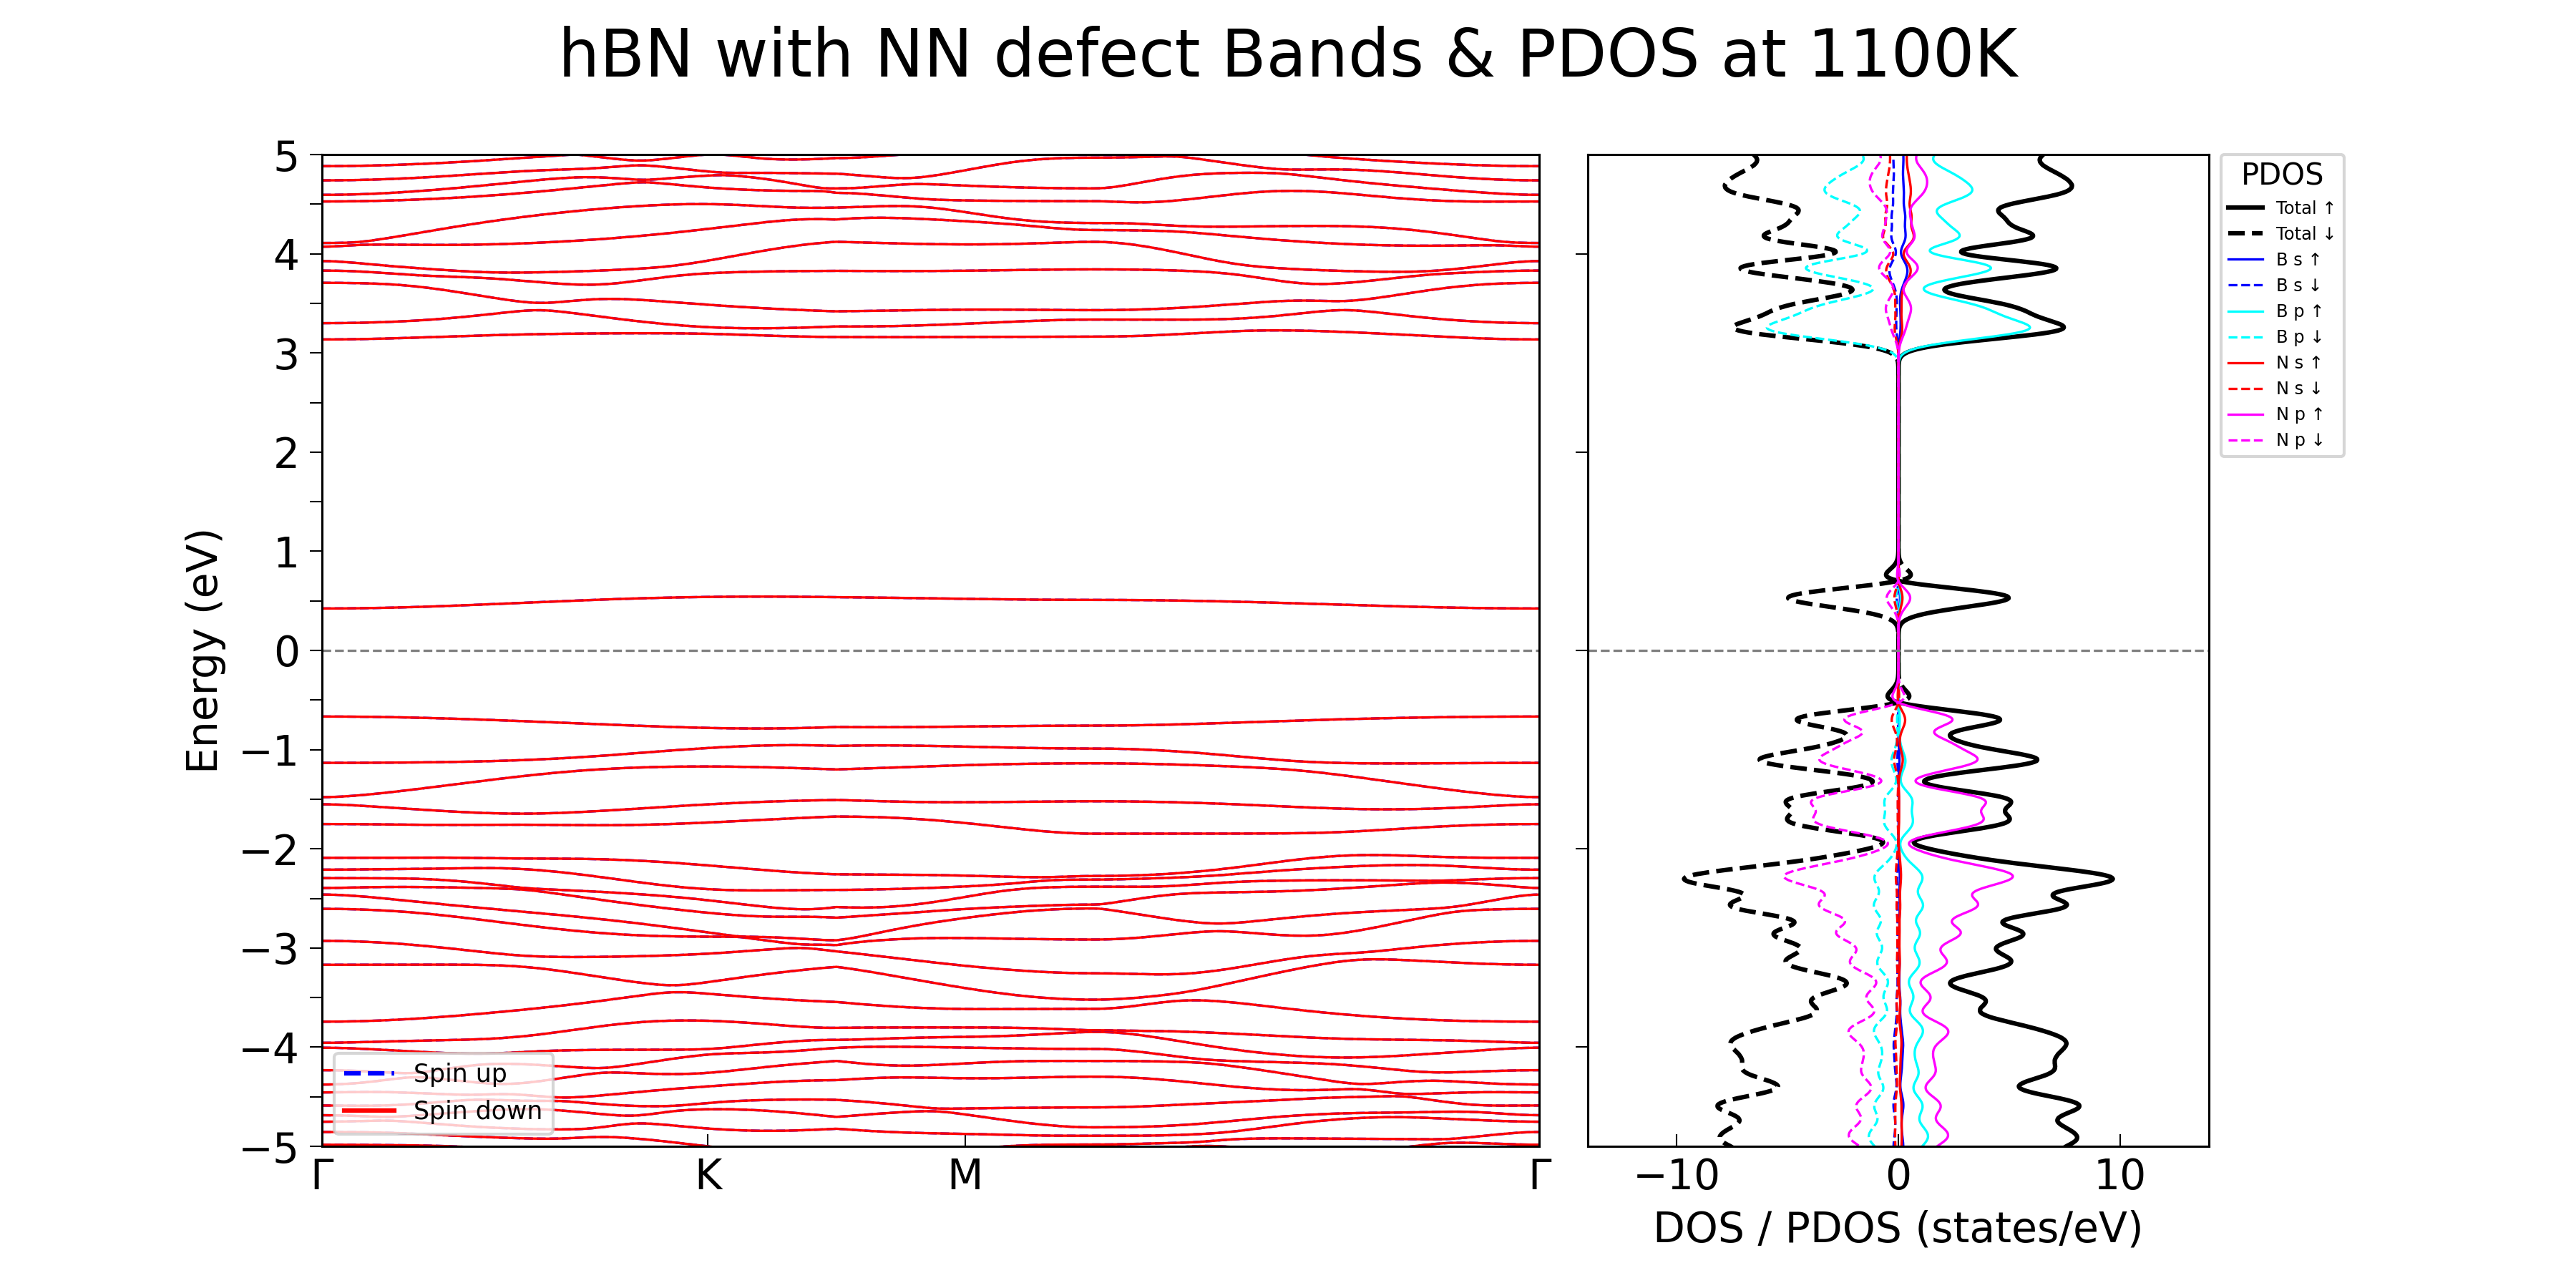
\includegraphics[width=0.9\textwidth]{gambar_hasil/simple_bands_pdos_NN_1100K.png}
    \caption{Struktur pita elektronik dan PDOS untuk monolayer hBN dengan defek N$_B$ pada 1100K.}
    \label{fig:hbn_NN_1100K}
\end{figure}
\begin{figure}[h!]
    \centering
    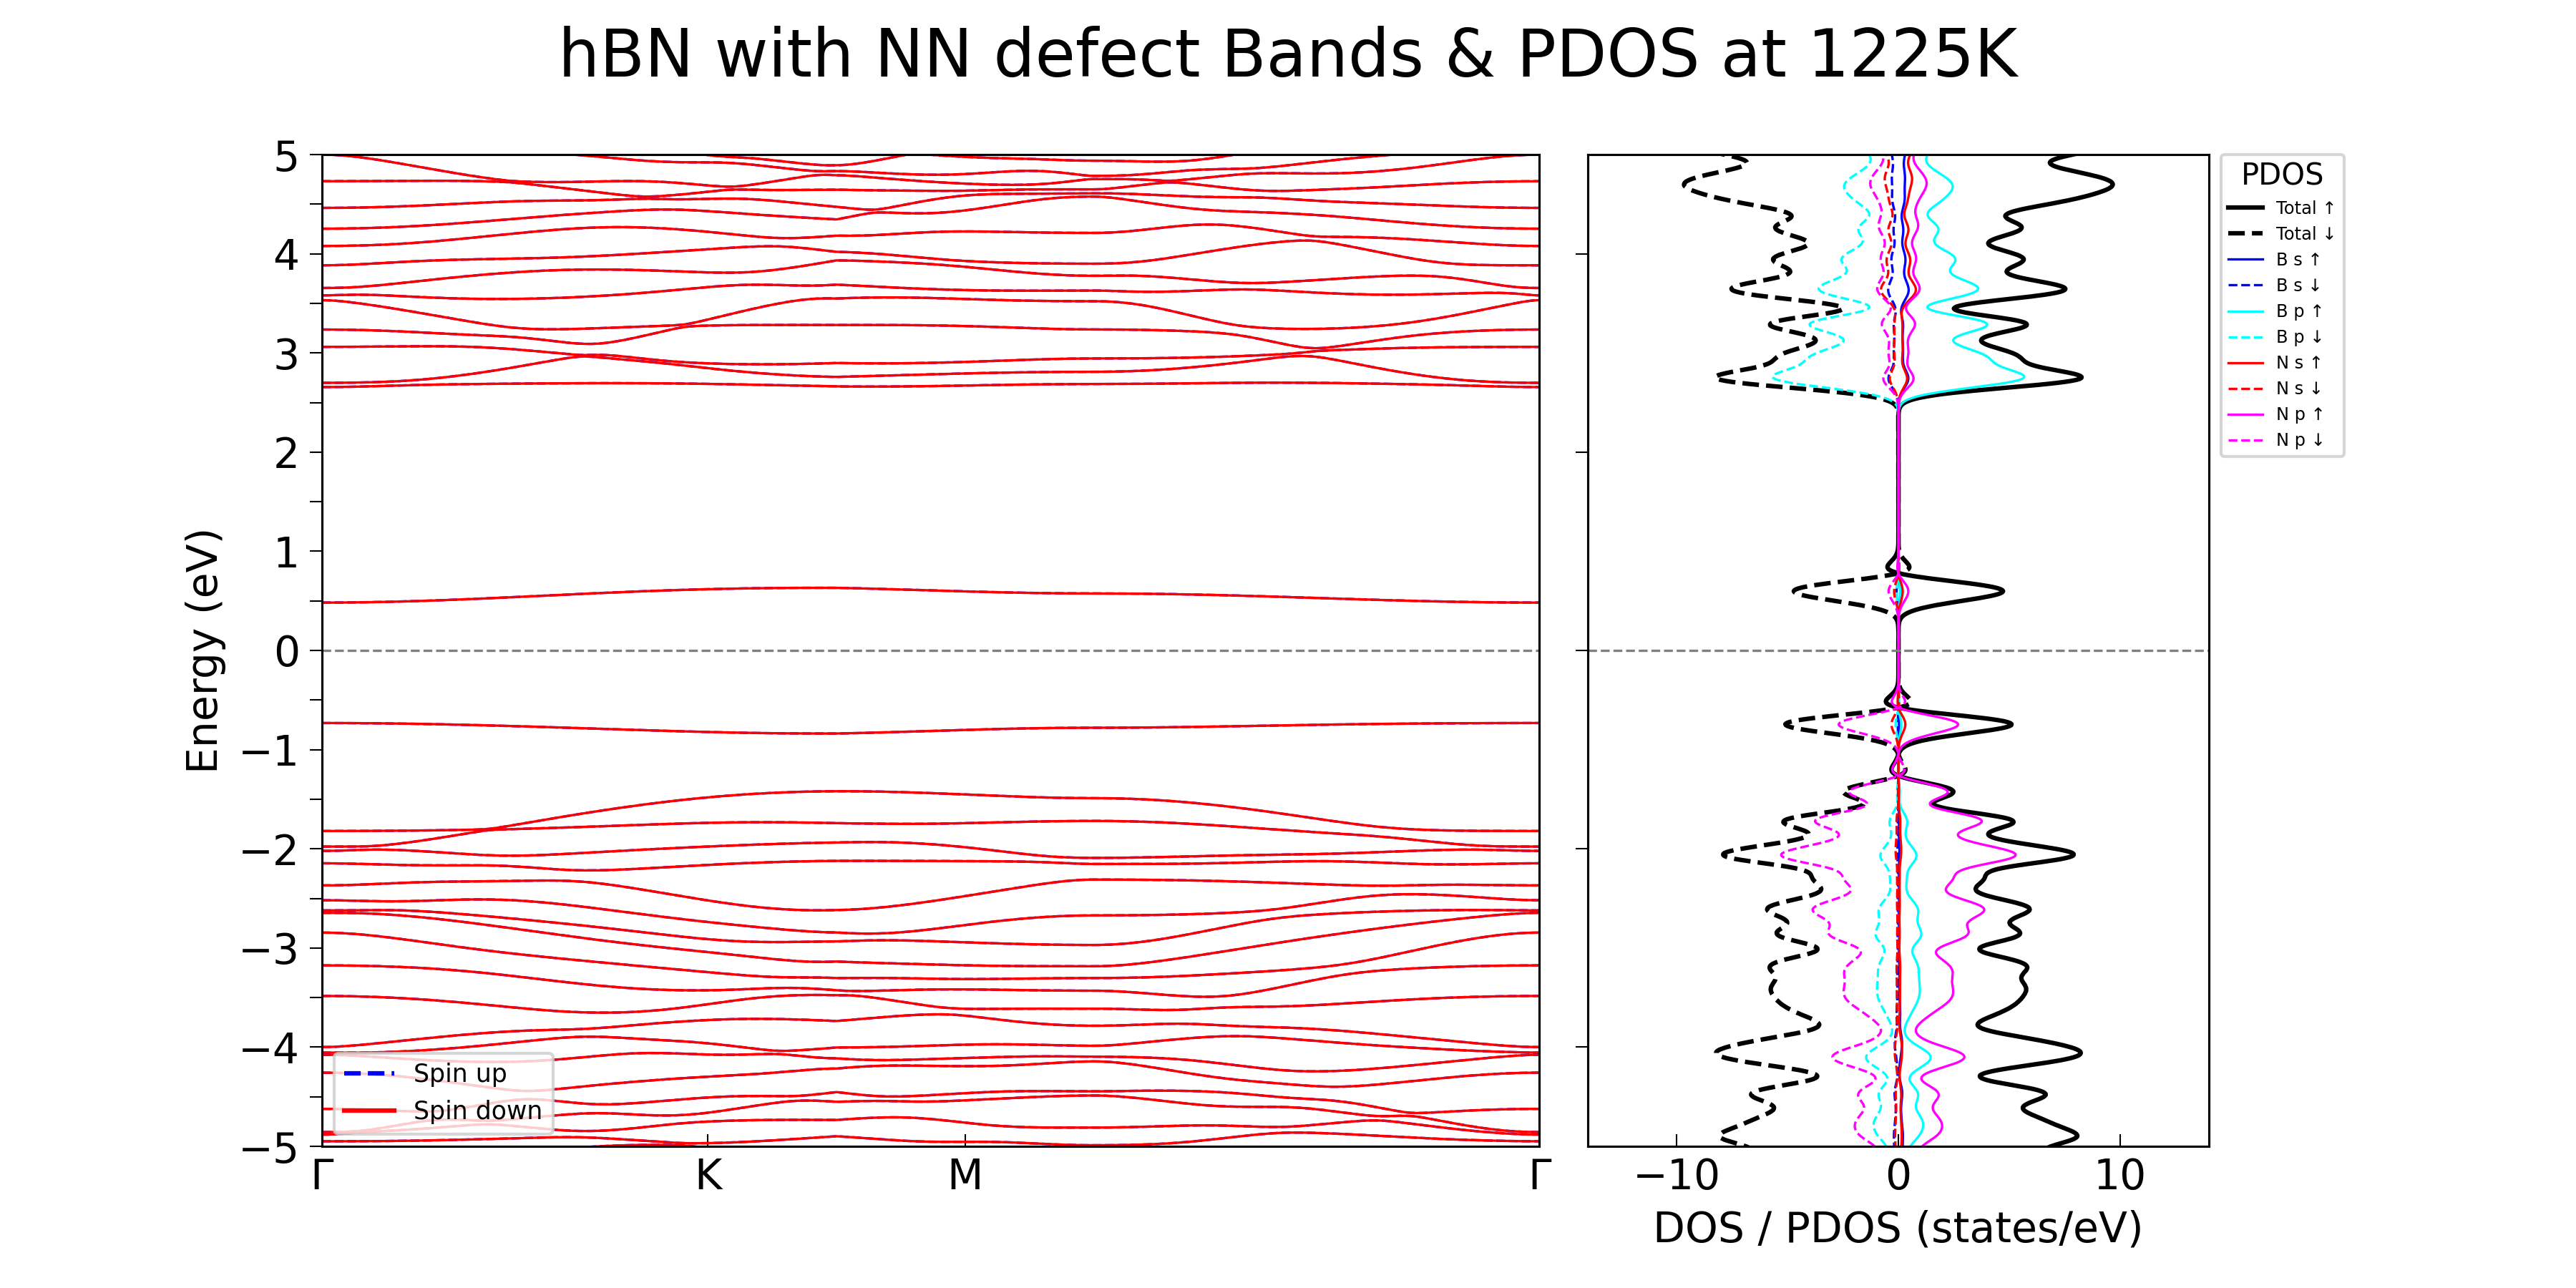
\includegraphics[width=0.9\textwidth]{gambar_hasil/simple_bands_pdos_NN_1225K.png}
    \caption{Struktur pita elektronik dan PDOS untuk monolayer hBN dengan defek N$_B$ pada 1225K.}
    \label{fig:hbn_NN_1225K}
\end{figure}
\begin{figure}[h!]
    \centering
    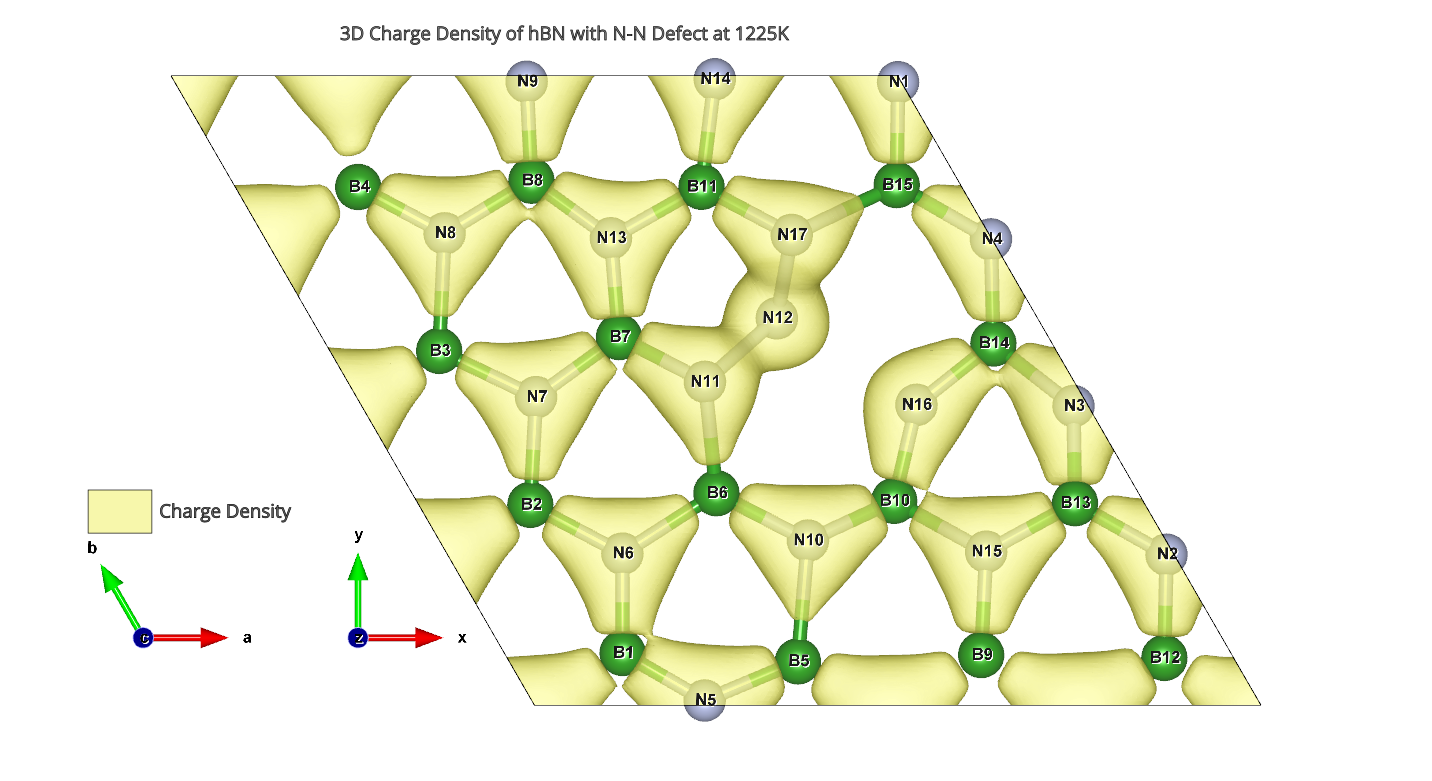
\includegraphics[width=0.6\textwidth]{gambar_hasil/hBN_rho_3D_NN_1225K.png}
    \caption{Visualisasi kerapatan muatan elektronik 3D untuk monolayer hBN dengan defek N$_B$ pada 1225K.}
    \label{fig:hbn_NN_1225K_chargedensity}
\end{figure}

Kehadiran defek N$_B$ menyebabkan reduksi celah pita energi ($E_g$) yang sangat drastis dibandingkan dengan hBN murni. Sebagai contoh, pada 800K, celah pita berkurang dari $4.415$ eV pada hBN murni menjadi hanya $0.694$ eV pada hBN dengan defek N$_B$ . Penurunan dramatis ini adalah konsekuensi langsung dari pembentukan tingkat-tingkat energi defek (\textit{defect states}) yang terlokalisasi secara spasial di sekitar situs defek N$_B$, yang muncul di dalam celah pita intrinsik hBN . Akibatnya, VBM dan CBM efektif dari sistem dengan defek ini sekarang ditentukan oleh posisi dari keadaan-keadaan defek tersebut, bukan lagi oleh pita valensi dan konduksi intrinsik hBN. Sebuah tren yang menarik dan tidak biasa teramati pada ketergantungan celah pita terhadap temperatur untuk sistem hBN+N$_B$: celah pita justru meningkat dengan kenaikan temperatur, dari $0.694$ eV pada 800K, menjadi $1.089$ eV pada 1100K, dan selanjutnya menjadi $1.214$ eV pada 1225K . Perilaku anomali ini berlawanan dengan tren penyempitan celah pita yang diamati pada hBN murni dan pada kebanyakan semikonduktor akibat efek EPC. Peningkatan celah pita dengan temperatur pada sistem yang mengandung defek N$_B$ ini menyiratkan bahwa keadaan-keadaan defek yang mendefinisikan VBM dan CBM efektif sangat sensitif terhadap distorsi struktural lokal di sekitar defek. Kenaikan temperatur menyebabkan perubahan pada distorsi ini, misalnya melalui relaksasi posisi atom-atom di sekitar N$_B$ atau perubahan panjang ikatan N-N atau N-B yang terbentuk di sekitar situs defek. Perubahan konfigurasi atomik ini, yang dipicu oleh temperatur, tampaknya mempengaruhi posisi relatif dari keadaan-keadaan defek tersebut sedemikian rupa sehingga celah energi efektif di antara mereka melebar. Hal ini dapat merupakan hasil dari interaksi yang kompleks antara defek dan vibrasi kisi (fonon) yang telah dimodifikasi oleh kehadiran defek itu sendiri, atau mungkin relaksasi struktural yang diinduksi temperatur di sekitar defek N$_B$ (misalnya, perubahan panjang ikatan N-N, atau geometri atom B di sekitarnya) mengubah energi keadaan defek. Jika relaksasi ini menyebabkan stabilisasi (penurunan energi) dari keadaan defek terisi (VBM baru) dan/atau destabilisasi (peningkatan energi) dari keadaan defek tak terisi (CBM baru), atau kombinasi yang meningkatkan pemisahan mereka, maka celah pita akan melebar . Implikasinya adalah bahwa sifat optoelektronik dari hBN yang mengandung defek N$_B$ akan menunjukkan ketergantungan temperatur yang unik dan berbeda secara kualitatif dari material induknya. Energi Fermi ($E_F$) juga mengalami pergeseran yang signifikan ke nilai yang jauh lebih negatif (misalnya, $-2.538$ eV pada 800K untuk hBN+N$_B$, dibandingkan dengan $-0.304$ eV pada 800K untuk hBN murni) . Pergeseran besar ini menunjukkan perubahan substansial dalam distribusi keadaan elektronik dan posisi tingkat okupansi tertinggi, yang kemungkinan besar disebabkan oleh pengisian elektron pada keadaan-keadaan defek yang baru terbentuk. Posisi Energi Fermi yang bergeser ini mengindikasikan bahwa defek N$_B$ dapat bertindak sebagai tingkat akseptor elektron, yang menjepit energi Fermi jauh di bagian bawah celah pita asli atau bagian atas pita valensi . \textbf{Sifat Magnetik:}
Untuk semua temperatur yang dikaji (800K, 1100K, 1225K), magnetisasi total dan magnetisasi absolut pada sistem hBN dengan defek N$_B$ tercatat sangat dekat dengan nol . Nilai magnetisasi absolut sebesar $0.010 \mu_B$ yang teramati pada 1225K kemungkinan besar berada dalam batas kebisingan numerik dari kalkulasi atau merepresentasikan efek magnetik yang sangat lemah dan dapat diabaikan . Momen orbital pada atom-atom juga tercatat nol.[1] Hasil ini mengindikasikan bahwa defek antisite N$_B$, pada konsentrasi dan kondisi struktur yang dipelajari (yaitu, struktur hasil relaksasi MD pada temperatur tinggi), tampaknya tidak menginduksi sifat magnetisme yang signifikan pada monolayer hBN. Temuan ini sejalan dengan sebagian besar literatur yang lebih sering mengaitkan defek N$_B$ dengan sifat optik daripada dengan induksi magnetisme. Sifat-sifat "defek NN" yang diamati (celah pita sangat kecil, ketergantungan suhu $E_g$ yang anomali) tidak mudah direkonsiliasi dengan literatur antisite N$_B$ yang sederhana dan terisolasi, yang sering melaporkan celah pita optik (ZPL) yang jauh lebih besar. Hal ini mungkin mengindikasikan bahwa "defek NN" dalam penelitian ini mewakili struktur defek kaya-Nitrogen yang lebih kompleks daripada N$_B$ tunggal, atau bahwa simulasi MD menghasilkan konfigurasi yang terdistorsi secara termal dengan ciri elektronik yang unik dan spesifik untuk kondisi simulasi tersebut. Istilah "defek NN" itu sendiri dapat menyiratkan adanya dua atom nitrogen dalam jarak dekat, seperti N$_B$ yang berdekatan dengan nitrogen interstisial (N$_i$), atau bahkan dimer N-N pada situs B. \subsection{Monolayer hBN dengan Defek Antisite B$_N$ ("BB defect")}
\label{subsec:hbn_defek_bn}
Defek antisite Boron (B$_N$), di mana atom Boron menempati situs atom Nitrogen, juga diharapkan akan mengubah lingkungan elektronik lokal secara signifikan. Literatur menyajikan gambaran yang beragam mengenai sifat cacat B$_N$. Beberapa studi teoritis menyarankan bahwa B$_N$ dalam keadaan netral (B$_N^0$) mungkin merupakan sumber foton tunggal non-magnetik dengan ZPL sekitar 1.58 eV. Namun, penelitian lain mengindikasikan bahwa defek secara umum di hBN, khususnya yang melibatkan atom Boron atau yang menciptakan ketidakseimbangan elektron valensi, berpotensi menginduksi magnetisme \citep{Zhang2020}. Data hasil kalkulasi untuk hBN dengan defek B$_N$ pada berbagai temperatur [1] dirangkum dalam Tabel \ref{tab:hbn_defek_bn} dan diilustrasikan pada Gambar \ref{fig:hbn_BB_800K} hingga \ref{fig:hbn_BB_1225K_spindensity}. \begin{table}[h!]
  \centering
  \caption{Sifat Elektronik dan Magnetik Monolayer hBN dengan Defek Antisite B$_N$ sebagai Fungsi Temperatur.}
  \label{tab:hbn_defek_bn}
  \resizebox{\textwidth}{!}{%
  \begin{tabular}{lcccccccccc}
    \toprule
    Temperatur & VBM & CBM & $E_g$ Sistem & $E_F$ & Mag. Total & Mag. Abs. & Momen Orbital & Momen Orbital & Momen Orbital & Momen Orbital \\
    (K) & (eV) & (eV) & Total (eV) & (eV) & ($\mu_B$) & ($\mu_B$) & B-s ($\mu_B$) & B-p ($\mu_B$) & N-s ($\mu_B$) & N-p ($\mu_B$) \\
    \midrule
    800  & -0.633          & 0.357           & 0.990 & -0.249 & 0.000 & 0.000 & -0.000 & 0.000 & -0.000 & 0.000 \\
    1100 
 & -0.120 ($\downarrow$) & 0.301 ($\uparrow$)  & 0.421 & -0.410 & 0.150 & 0.230 &  0.003 & 0.010 & -0.000 & 0.001 \\
    1225 & -0.073 ($\uparrow$) & 0.243 ($\downarrow$)  & 0.316 & -0.622 & 1.850 & 2.320 &  0.057 & 0.009 & -0.022 & -0.002 \\
    \bottomrule
  \end{tabular}%
  }
\end{table}

\begin{figure}[h!]
    \centering
    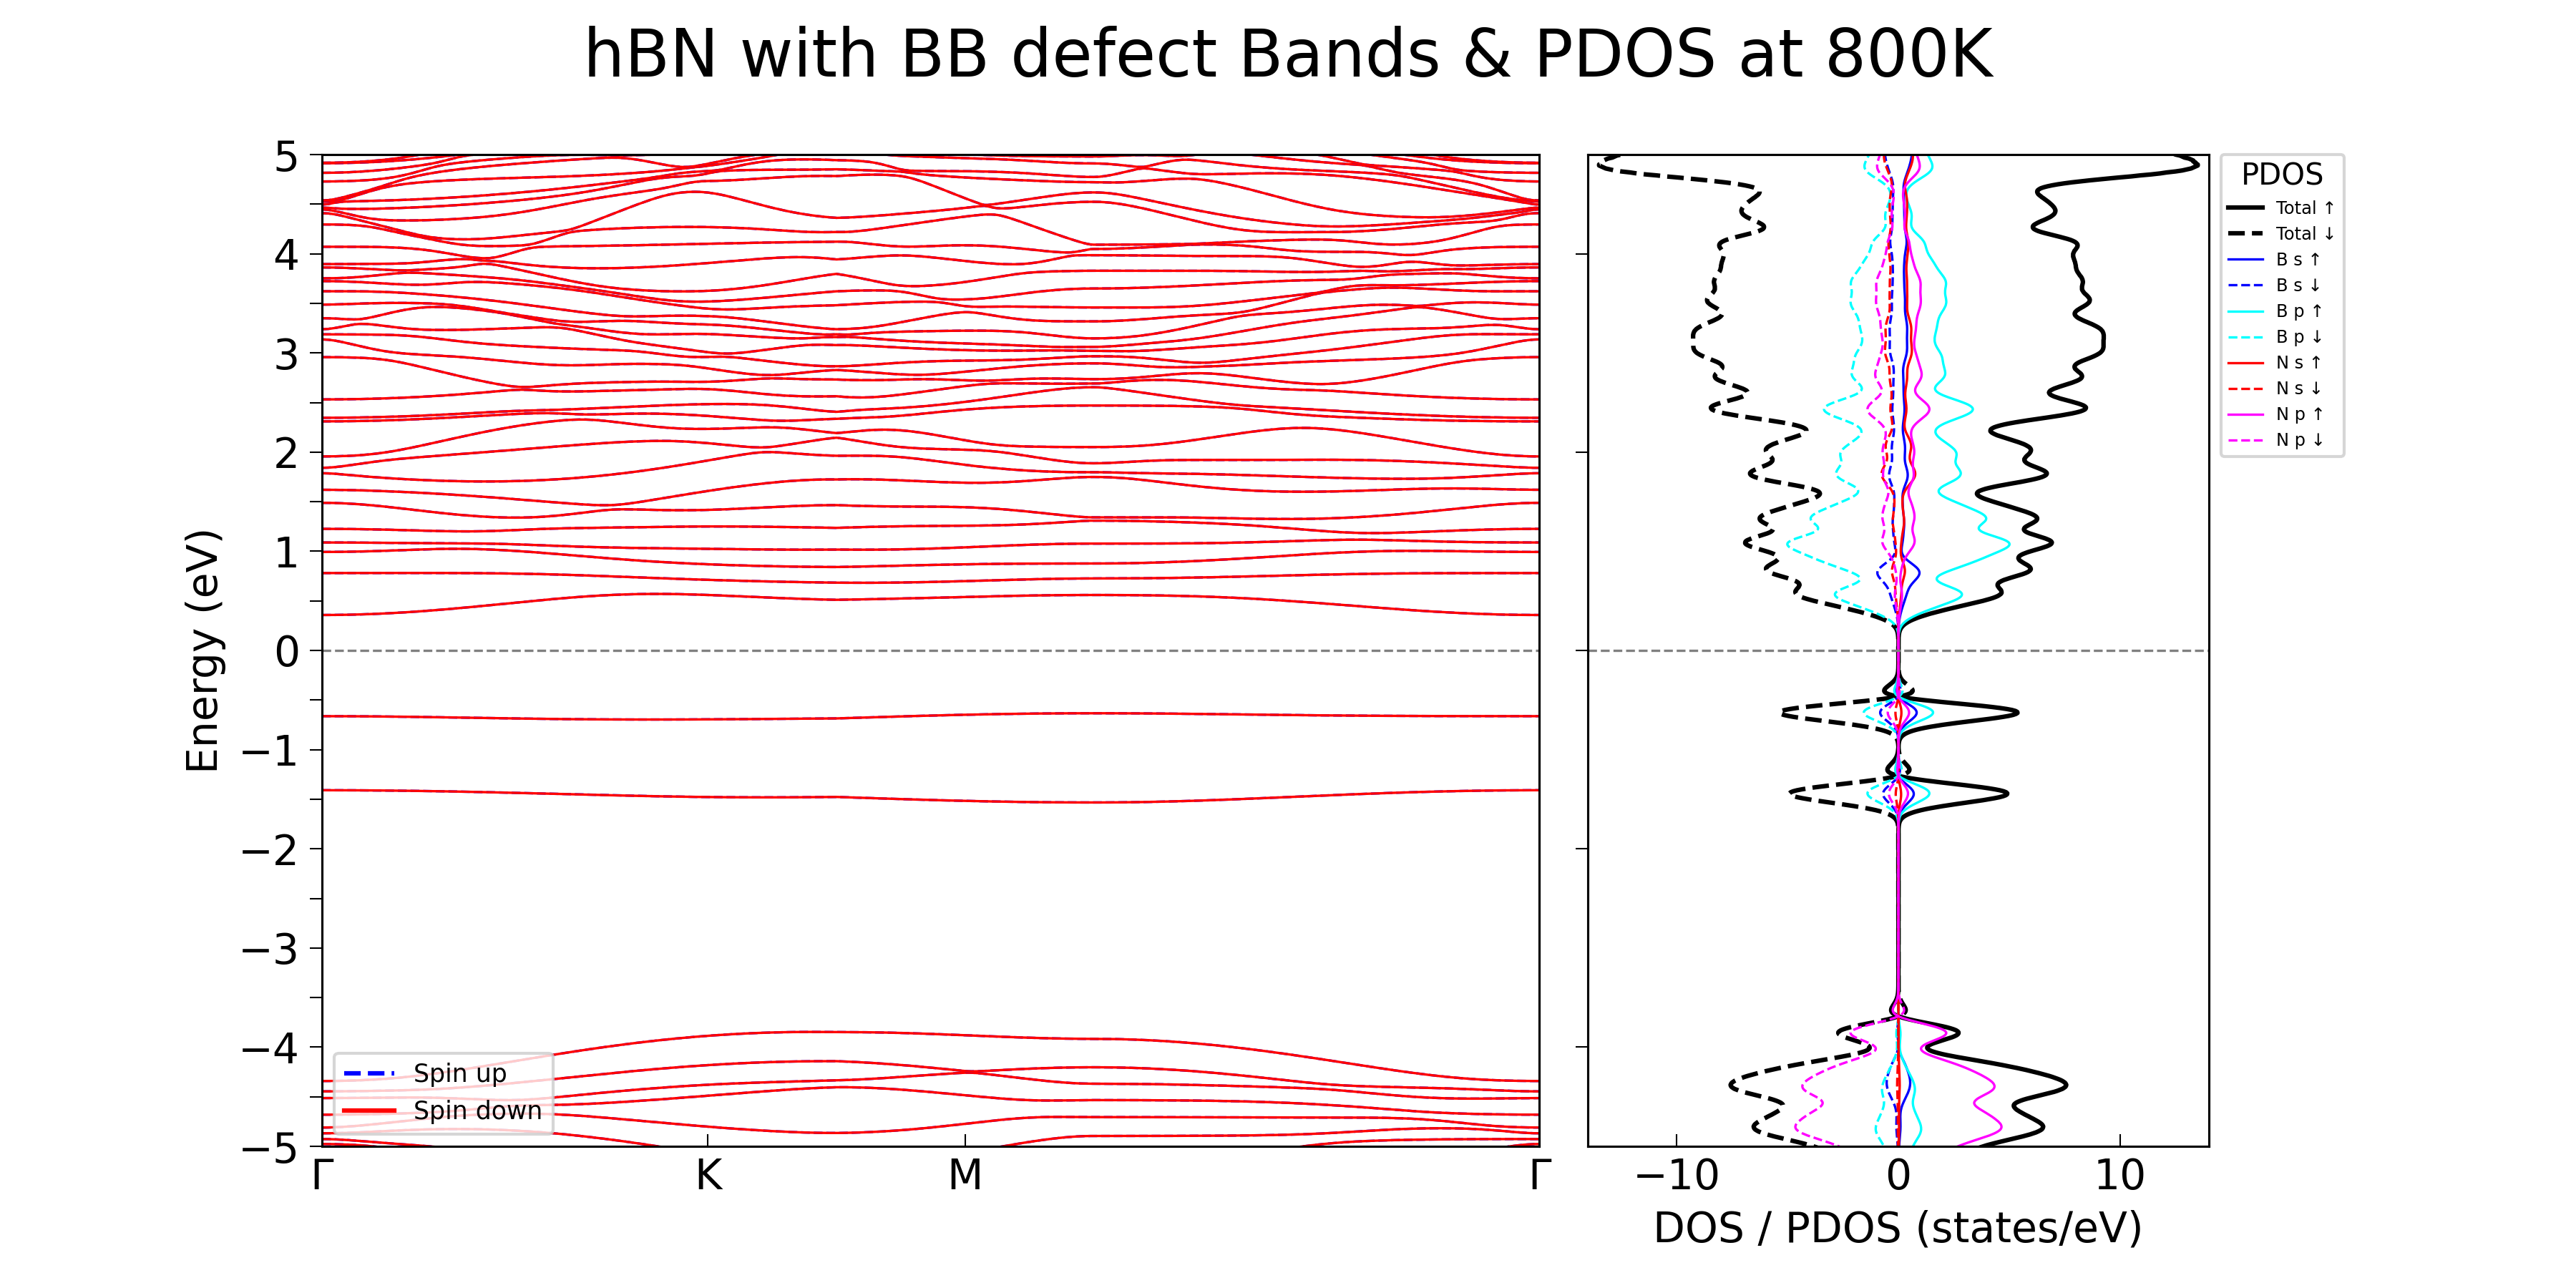
\includegraphics[width=0.9\textwidth]{gambar_hasil/simple_bands_pdos_BB_800K.png}
    \caption{Struktur pita elektronik dan PDOS untuk monolayer hBN dengan defek B$_N$ pada 800K.}
    \label{fig:hbn_BB_800K}
\end{figure}
\begin{figure}[h!]
    \centering
    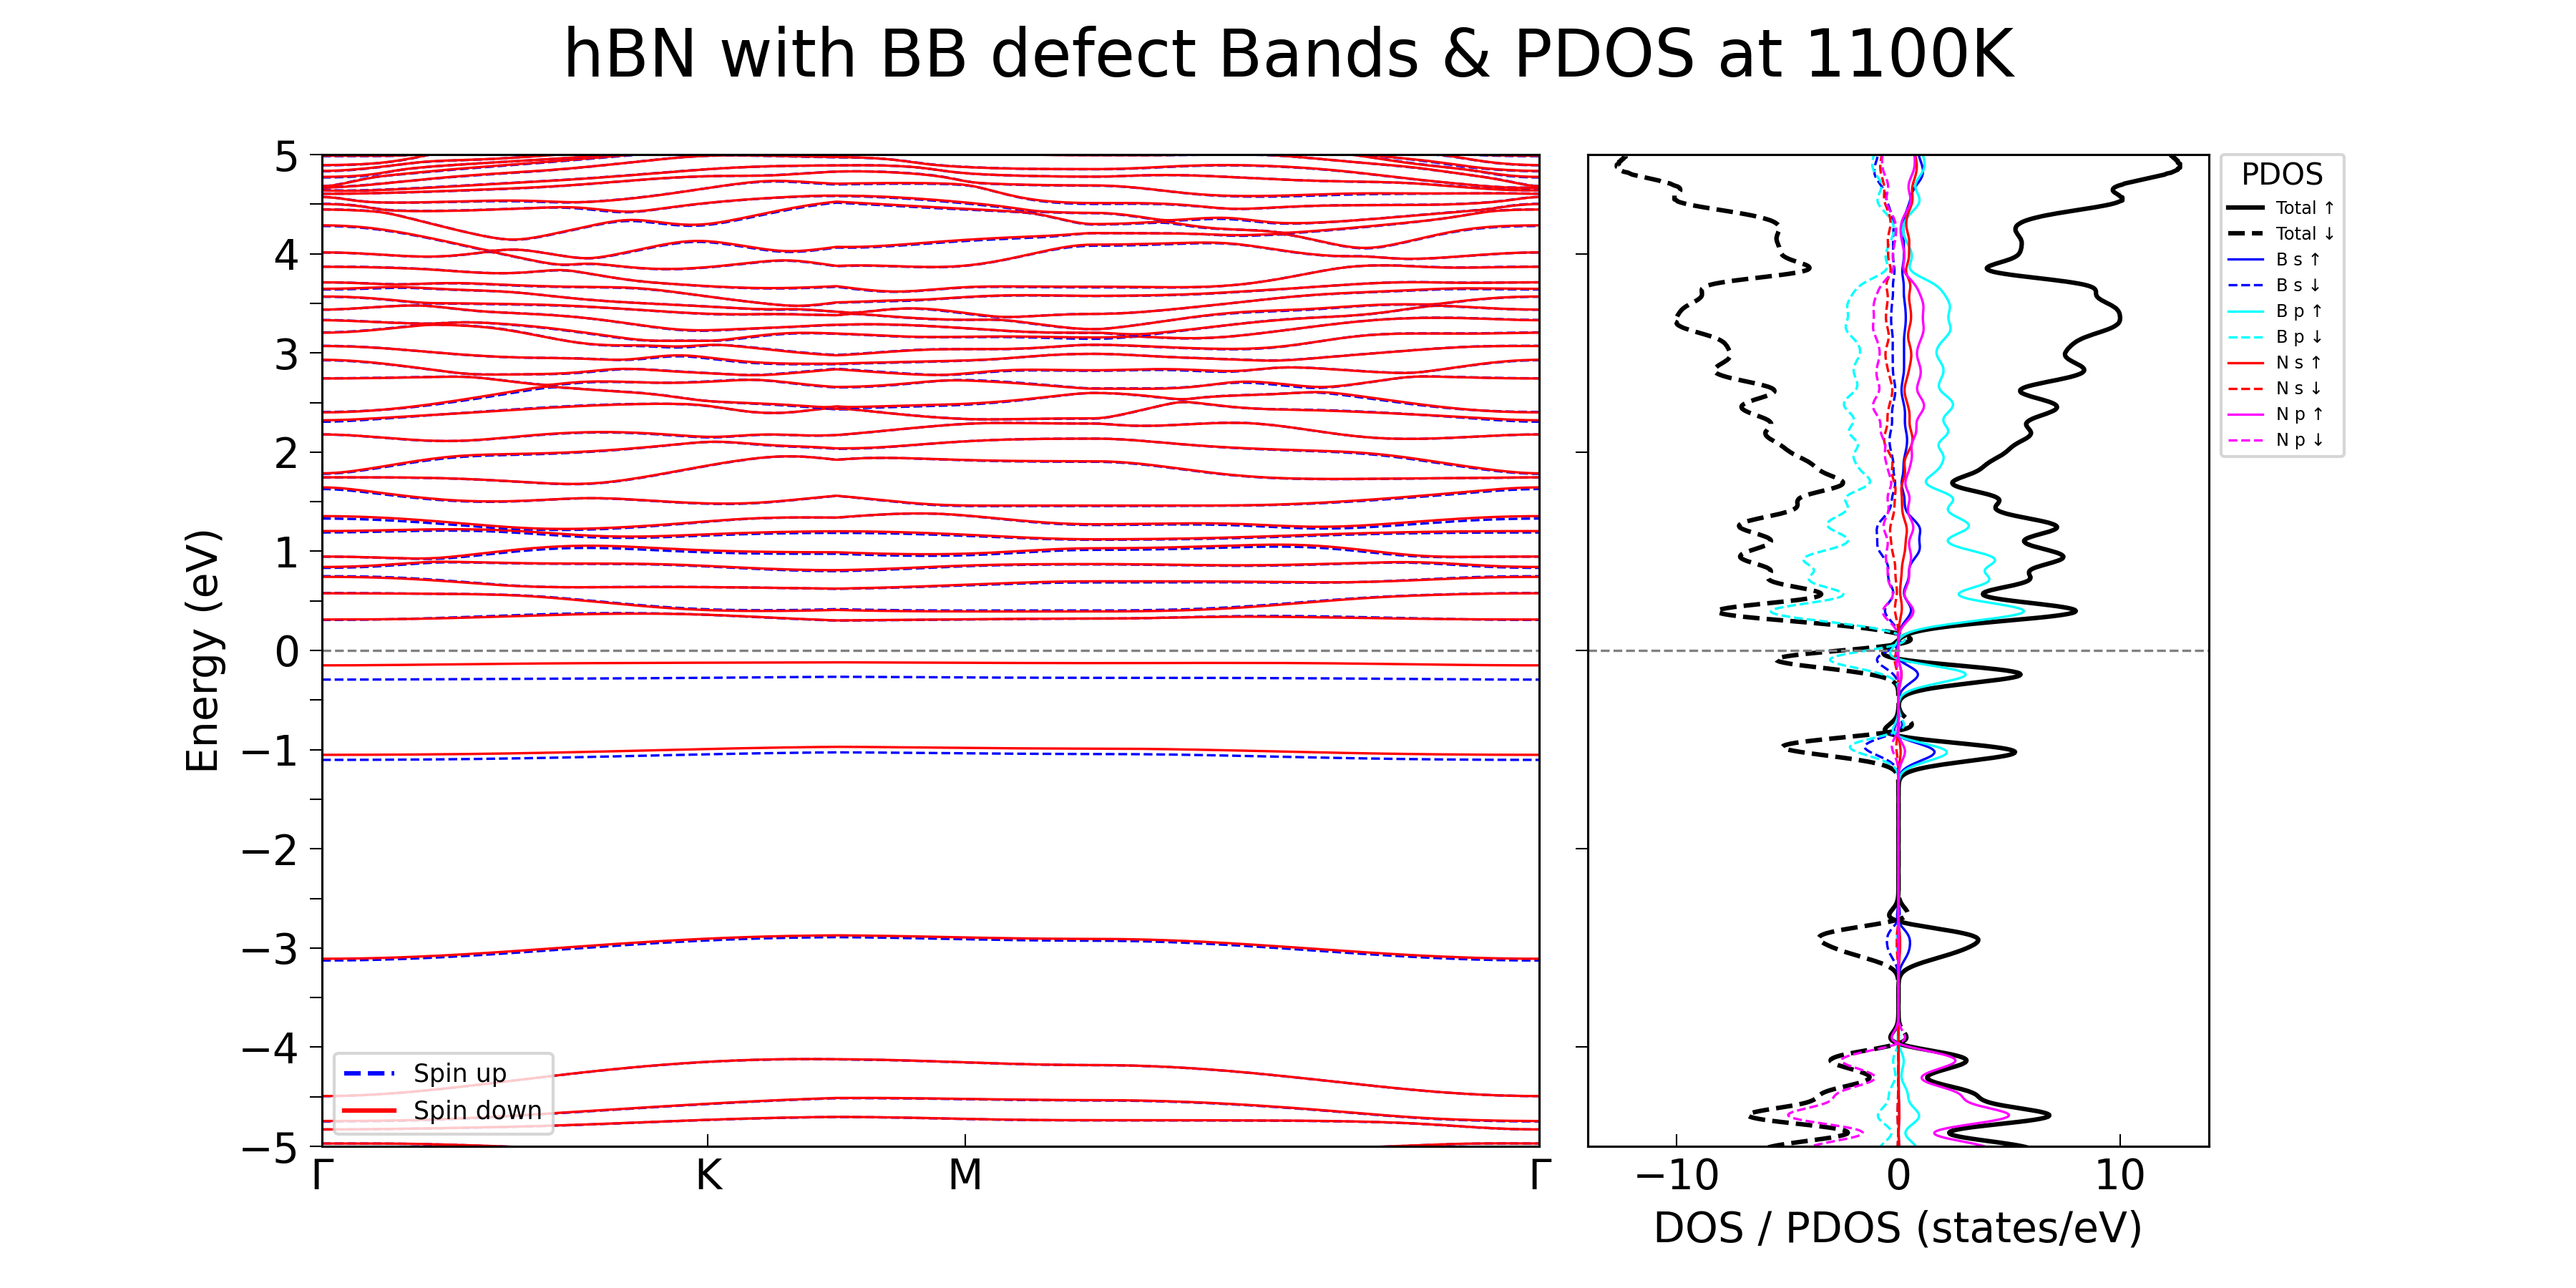
\includegraphics[width=0.9\textwidth]{gambar_hasil/simple_bands_pdos_BB_1100K.png}
    \caption{Struktur pita elektronik dan PDOS untuk monolayer hBN dengan defek B$_N$ pada 1100K, menunjukkan pemisahan spin.}
    \label{fig:hbn_BB_1100K}
\end{figure}
\begin{figure}[h!]
    \centering
    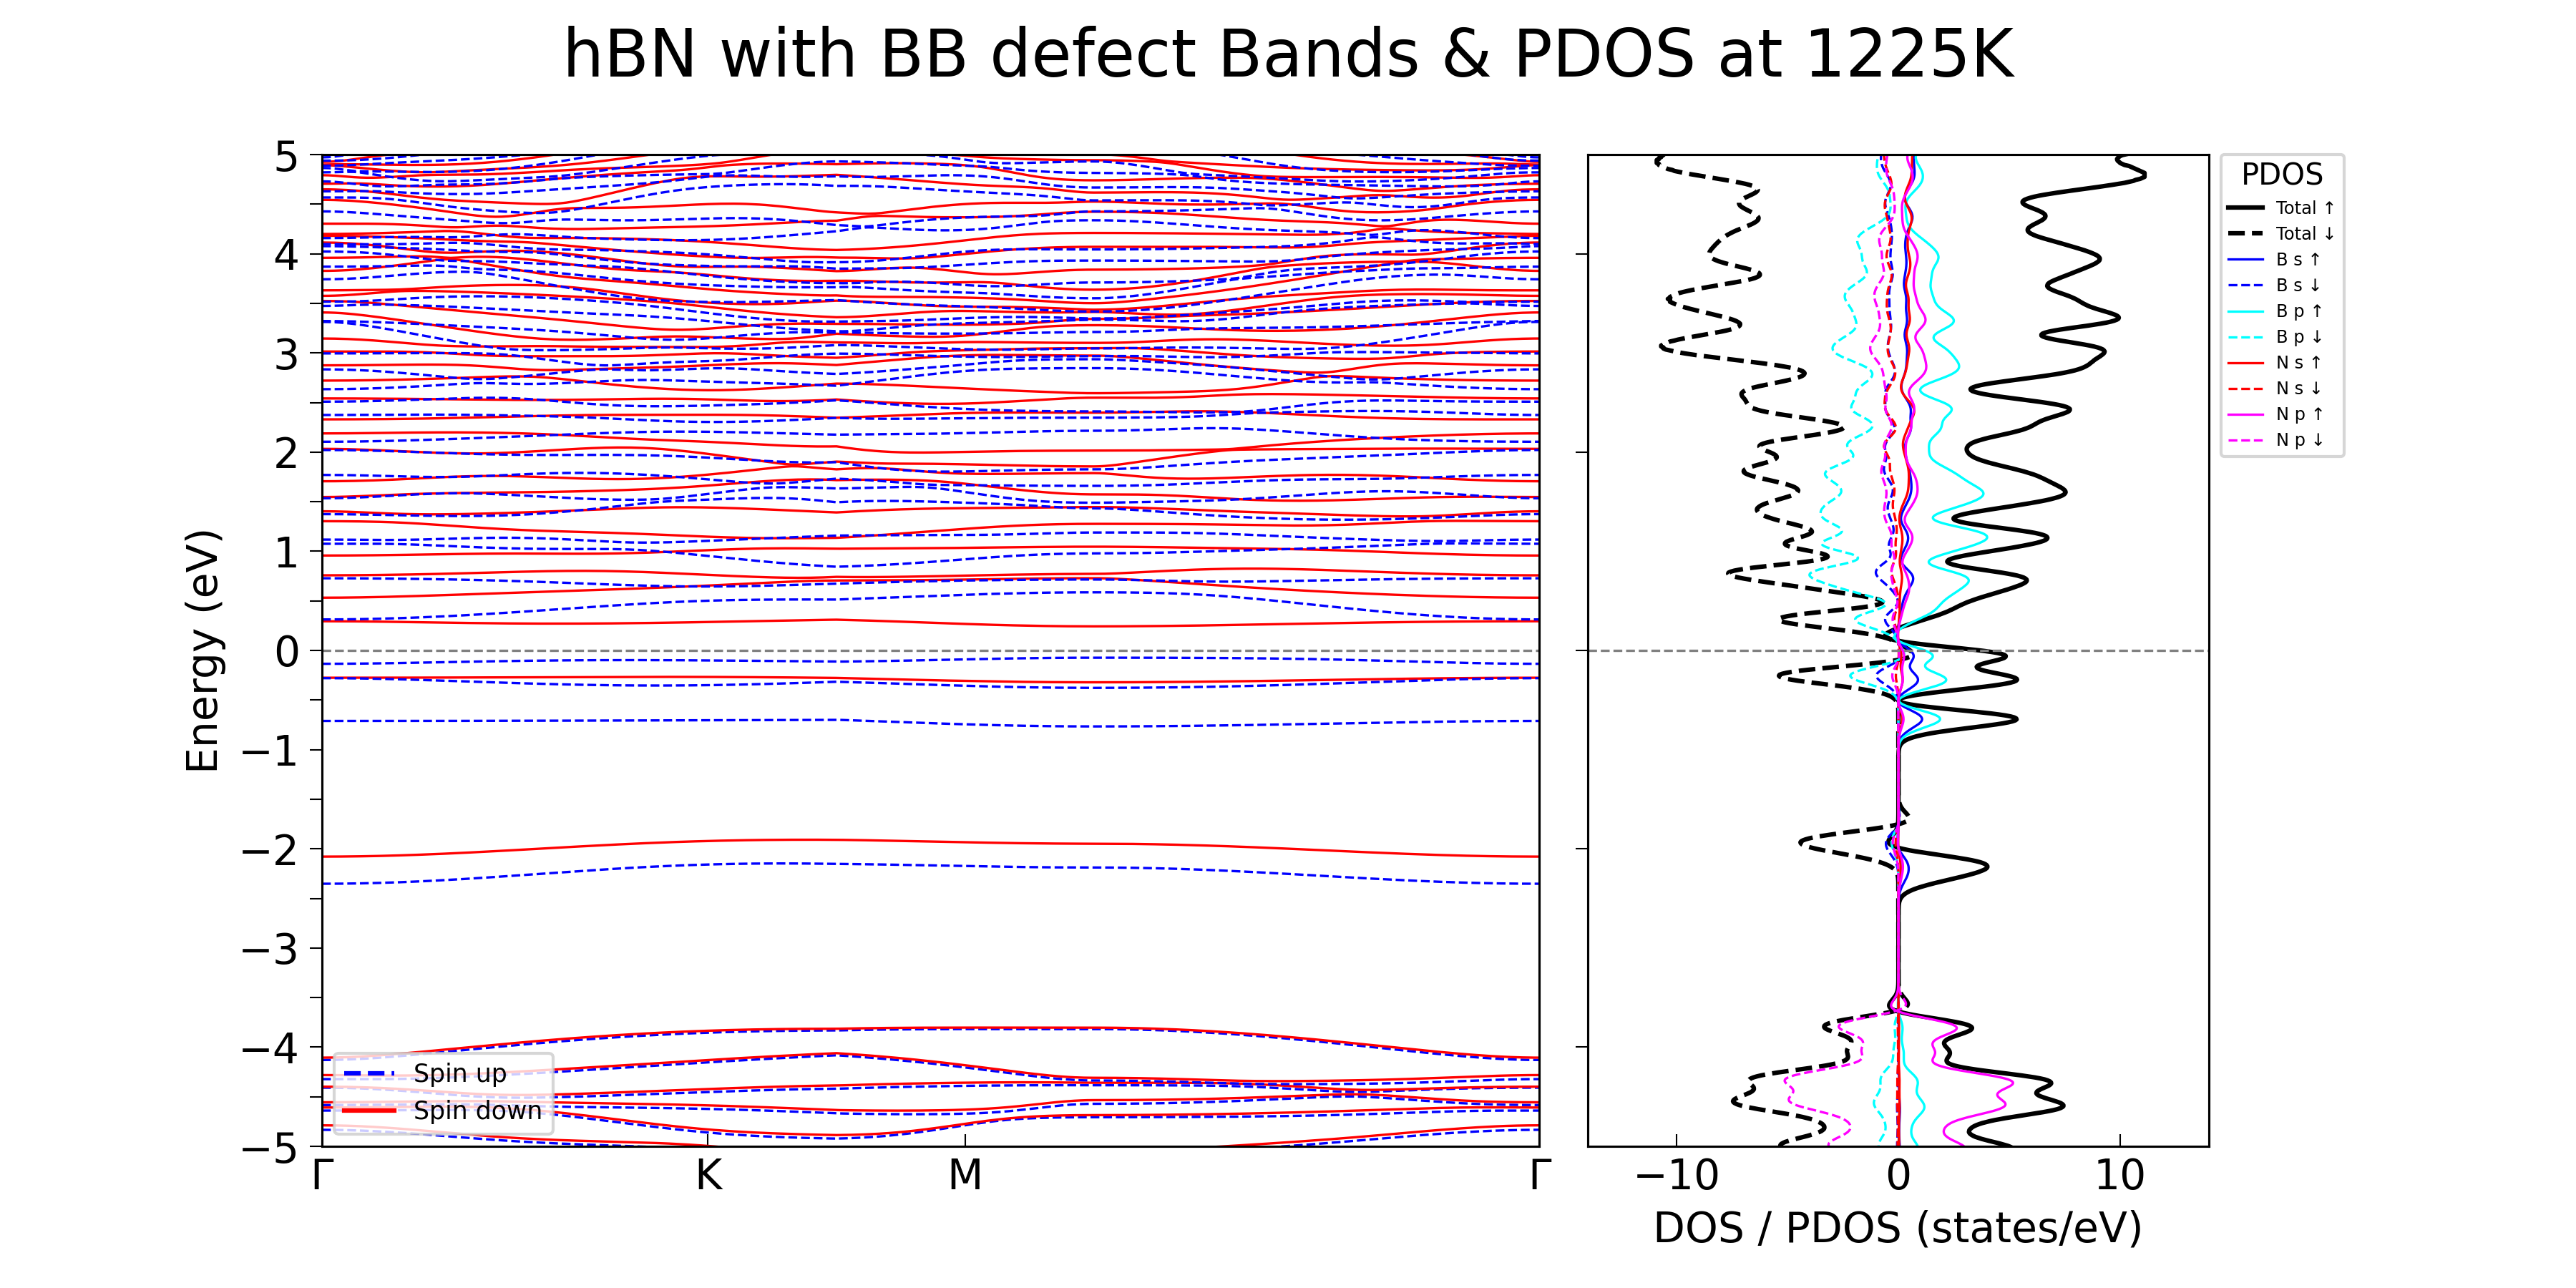
\includegraphics[width=0.9\textwidth]{gambar_hasil/simple_bands_pdos_BB_1225K.png}
    \caption{Struktur pita elektronik dan PDOS untuk monolayer hBN dengan defek B$_N$ pada 1225K, menunjukkan pemisahan spin yang lebih signifikan.}
    \label{fig:hbn_BB_1225K}
\end{figure}
\begin{figure}[h!]
    \centering
    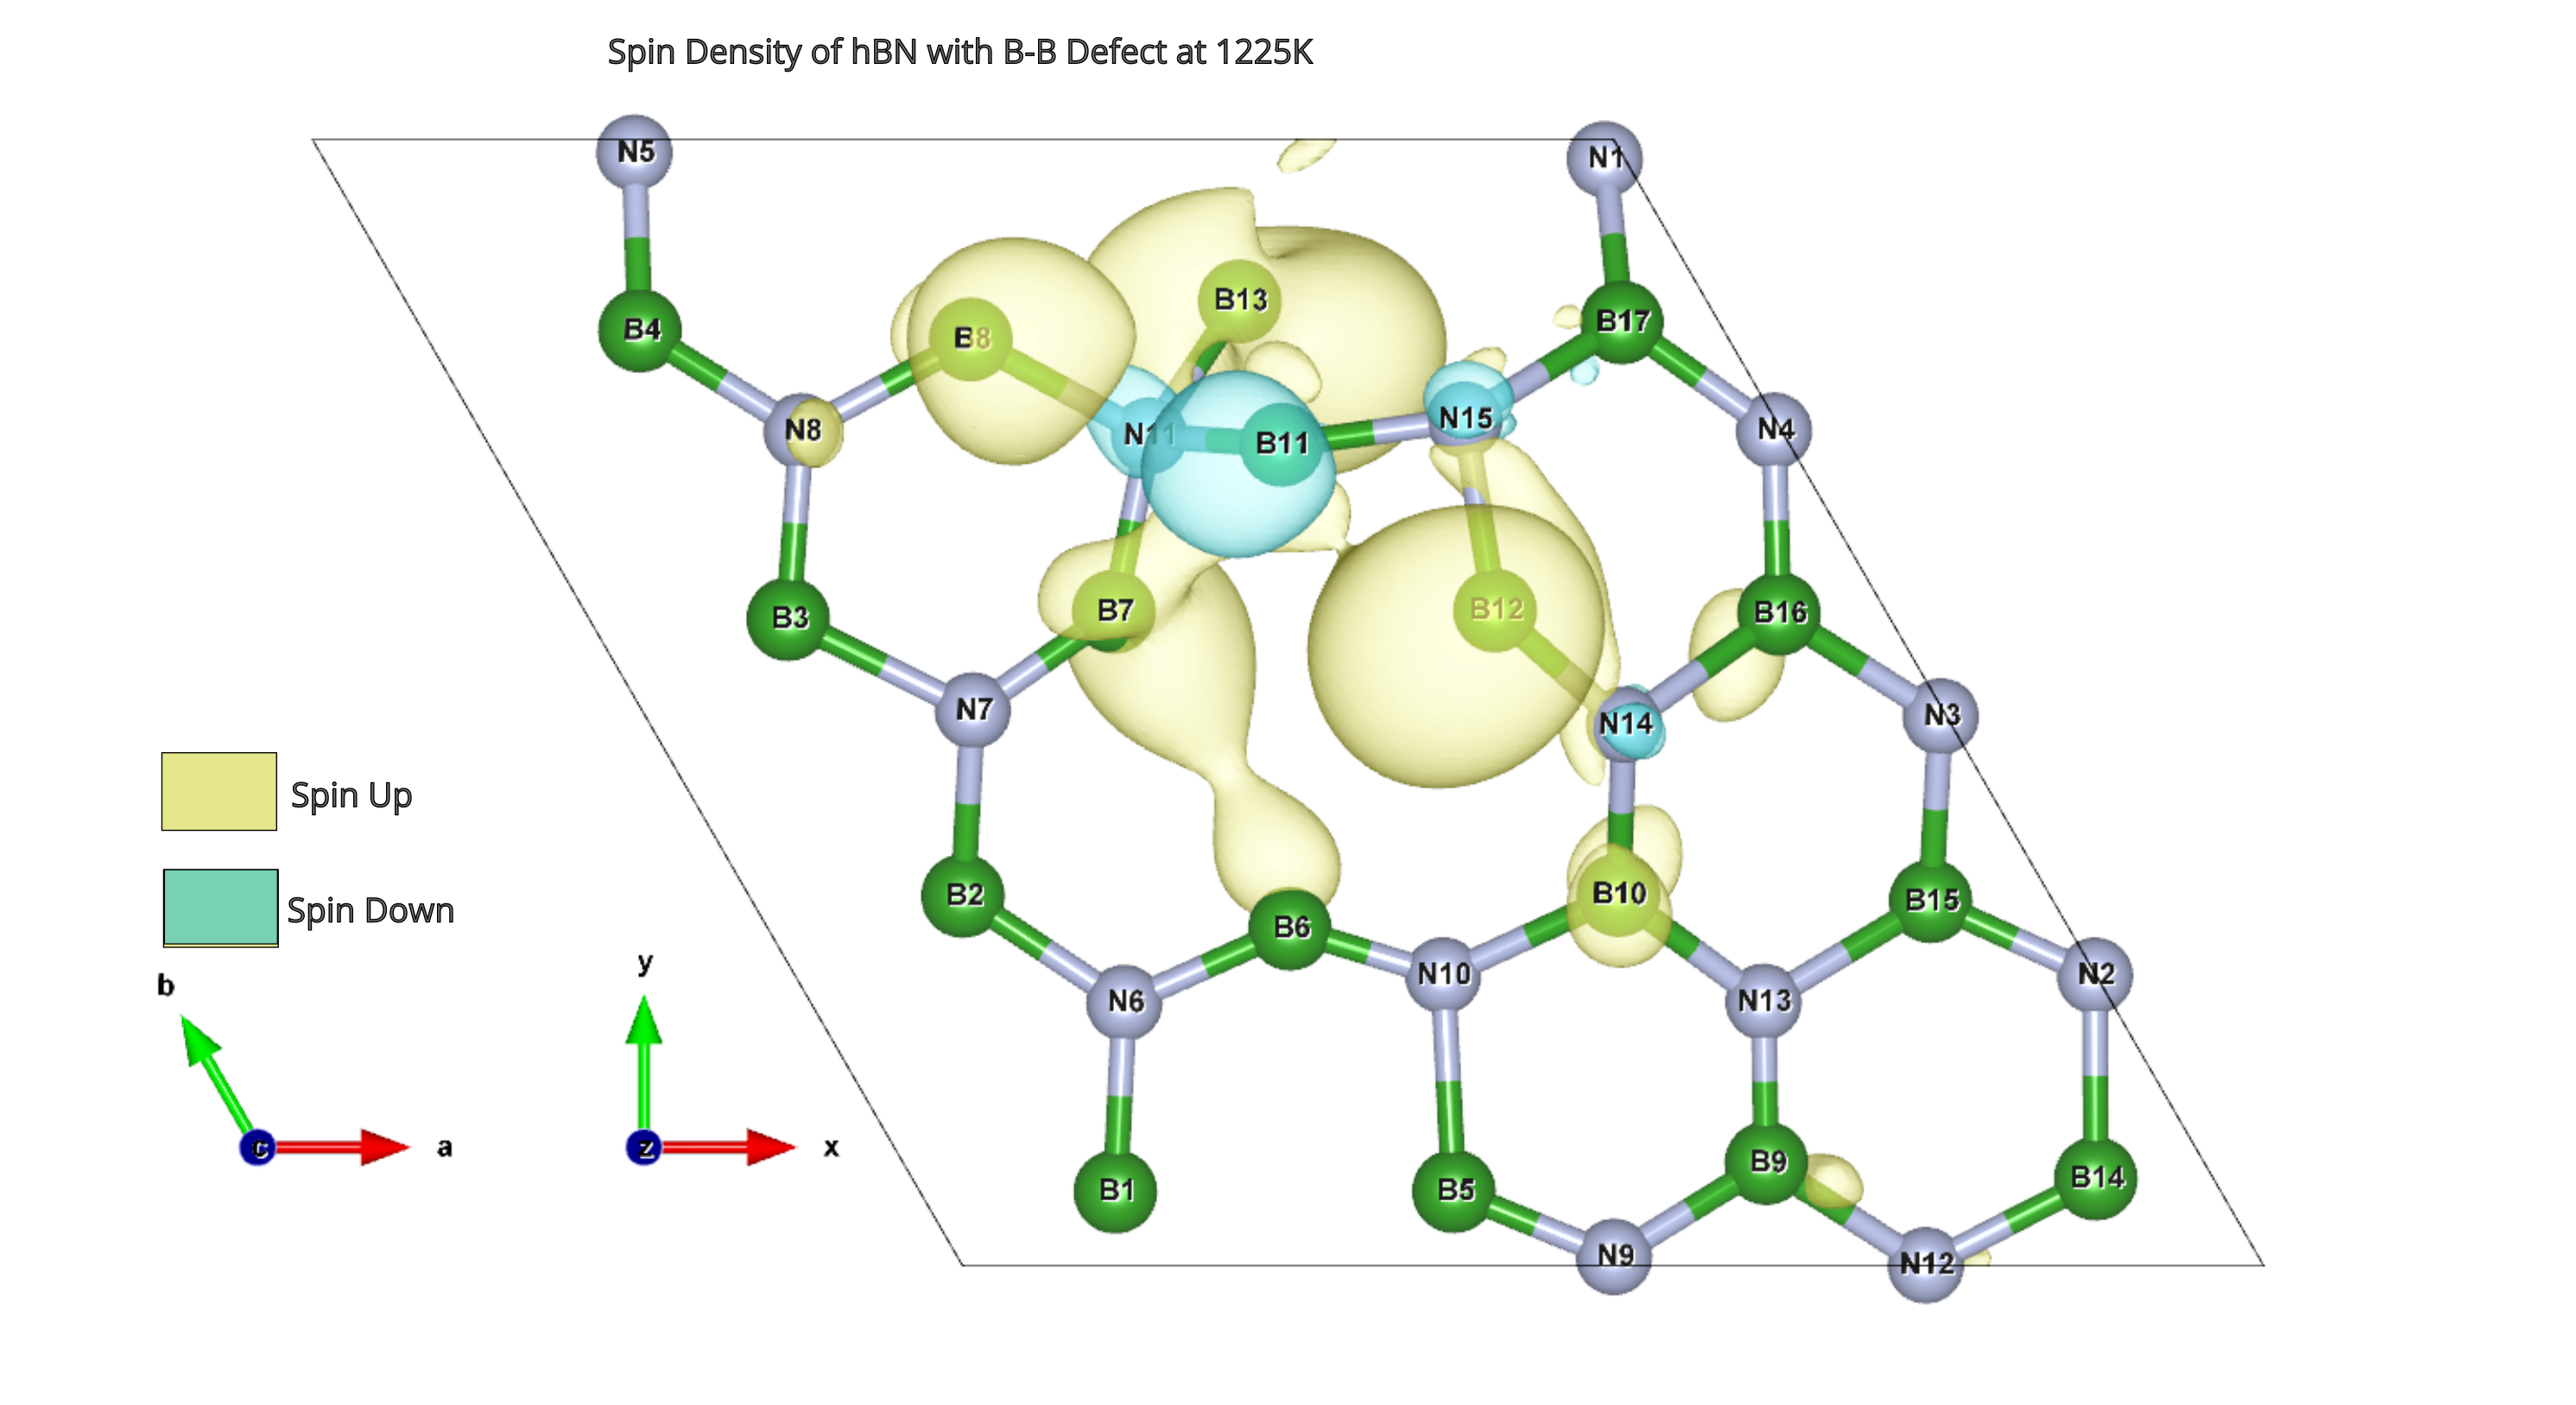
\includegraphics[width=0.6\textwidth]{gambar_hasil/hBN_spin_BB_1225K.png}
    \caption{Visualisasi kerapatan spin 3D untuk monolayer hBN dengan defek B$_N$ pada 1225K, menunjukkan lokalisasi momen magnetik.}
    \label{fig:hbn_BB_1225K_spindensity}
\end{figure}
% Placeholder untuk gambar kerapatan muatan B_N jika ada di [1]
% \begin{figure}[h!]
%     \centering
%     \includegraphics[width=0.6\textwidth]{placeholder_[1]_page10_chargedensity_BB_1225K.png}
%     \caption{Visualisasi kerapatan muatan elektronik 3D untuk monolayer hBN dengan defek B$_N$ pada 1225K. [1]}
%     \label{fig:hbn_BB_1225K_chargedensity}
% \end{figure}

\textbf{Perubahan Struktur Elektronik:}
Serupa dengan kasus defek N$_B$, kehadiran defek B$_N$ juga mengintroduksi keadaan-keadaan defek yang signifikan di dalam celah pita intrinsik hBN, yang dapat diamati dari plot DOS. Celah pita sistem total untuk hBN dengan defek B$_N$ menunjukkan tren penurunan dengan kenaikan temperatur: dari $0.990$ eV pada 800K, menjadi $0.421$ eV pada 1100K, dan selanjutnya menjadi $0.316$ eV pada 1225K . Tren penurunan celah pita dengan temperatur ini serupa dengan yang diamati pada hBN murni, tetapi berbeda dengan perilaku pada hBN dengan defek N$_B$ (yang menunjukkan peningkatan). Hal ini menyiratkan bahwa mekanisme yang mengatur perubahan celah pita dengan temperatur untuk sistem dengan defek B$_N$ mungkin lebih mirip dengan material induknya atau didominasi oleh efek yang berbeda dibandingkan dengan sistem yang mengandung defek N$_B$. Energi Fermi juga mengalami pergeseran dan nilainya bervariasi dengan temperatur: $-0.249$ eV pada 800K, $-0.410$ eV pada 1100K, dan $-0.622$ eV pada 1225K . Pergeseran ini, bersamaan dengan munculnya sifat magnetik, menunjukkan modifikasi besar pada lanskap elektronik sistem akibat defek B$_N$ dan pengaruh temperatur. Perbedaan mencolok mulai terlihat pada temperatur 1100K dan 1225K. Pada kedua temperatur ini, terlihat adanya pemisahan spin (\textit{spin splitting}) yang jelas pada DOS, terutama di sekitar Energi Fermi (Gambar \ref{fig:hbn_BB_1100K} dan \ref{fig:hbn_BB_1225K}). Ini mengindikasikan bahwa sistem menjadi magnetik. Struktur pita energi juga akan menunjukkan perbedaan antara kanal spin-atas (\textit{spin-up}) dan spin-bawah (\textit{spin-down}), yang mengarah pada celah pita yang berbeda untuk masing-masing spin. Sebagai contoh, pada 1100K, VBM sistem (-0.120 eV) ditentukan oleh kanal spin-bawah, sedangkan CBM sistem (0.301 eV) ditentukan oleh kanal spin-atas. Pada 1225K, VBM sistem (-0.073 eV) ditentukan oleh kanal spin-atas, dan CBM sistem (0.243 eV) oleh kanal spin-bawah . \textbf{Sifat Magnetik yang Terinduksi dan Asal Usulnya:}
Perilaku magnetik sistem hBN dengan defek B$_N$ menunjukkan ketergantungan yang kuat terhadap temperatur. Pada 800K, sistem ini tidak menunjukkan magnetisasi yang signifikan (Magnetisasi Total dan Absolut tercatat $0.000 \mu_B$) dan momen orbital pada atom-atom juga nol . Namun, pada 1100K, sistem mulai menunjukkan sifat magnetik dengan magnetisasi total terukur sebesar $0.150 \mu_B$ dan magnetisasi absolut sebesar $0.230 \mu_B$. Perbedaan antara nilai total dan absolut ini mengindikasikan kemungkinan adanya konfigurasi spin yang tidak sepenuhnya feromagnetik, misalnya beberapa momen magnetik lokal mungkin tersusun secara anti-sejajar atau membentuk struktur spin yang lebih kompleks . Lebih lanjut, momen orbital juga teramati pada atom Boron (B-s = $0.003 \mu_B$, B-p = $0.010 \mu_B$), yang mengkonfirmasi munculnya respons magnetik . Pada 1225K, sifat magnetik menjadi jauh lebih jelas dan kuat. Magnetisasi total meningkat secara signifikan menjadi $1.850 \mu_B$, dan magnetisasi absolut menjadi $2.320 \mu_B$. Momen orbital pada orbital $s$ atom Boron (B-s) juga meningkat menjadi $0.057 \mu_B$, sementara momen orbital juga terdeteksi pada orbital $s$ atom Nitrogen (N-s = $-0.022 \mu_B$) . Ini menunjukkan penguatan sifat magnetik pada temperatur yang lebih tinggi. Kemunculan magnetisme pada sistem hBN dengan defek B$_N$ pada temperatur tinggi (1100K dan 1225K) merupakan temuan yang sangat menarik, terutama jika dikontraskan dengan beberapa laporan literatur yang menyarankan bahwa defek B$_N$ dalam keadaan netral (B$_N^0$) bersifat non-magnetik pada perhitungan 0K. Perbedaan ini dapat dipahami melalui beberapa pertimbangan. Pertama, pengaruh temperatur dan distorsi struktur: struktur atomik yang digunakan dalam kalkulasi DFT ini berasal dari simulasi MD pada temperatur tinggi. Distorsi termal dan relaksasi struktur yang terjadi di sekitar defek B$_N$ pada temperatur tersebut mungkin mengubah simetri lokal dan konfigurasi elektronik secara signifikan dibandingkan dengan struktur B$_N^0$ yang dioptimasi pada 0K. Perubahan simetri ini dapat memecah degenerasi orbital-orbital atom, yang kemudian mengarah pada pengisian elektron yang tidak seimbang antara kanal spin-atas dan spin-bawah, sehingga menghasilkan momen magnetik netto . Kedua, pembentukan ikatan B-B atau kluster Boron lokal: adanya defek B$_N$ berarti sebuah atom Boron dikelilingi oleh tiga atom Boron tetangga (jika defek B$_N$ menggantikan atom Nitrogen yang terikat pada atom Boron normal dalam kisi hBN). Interaksi antar atom Boron ini, atau pembentukan ikatan B-B lokal, dapat memiliki sifat elektronik dan magnetik yang unik. Magnetisme yang teramati kemungkinan besar adalah feromagnetisme $d^0$, karena hBN tidak mengandung unsur dengan elektron $d$ yang biasanya bertanggung jawab atas magnetisme konvensional . Jenis magnetisme ini timbul dari polarisasi spin elektron $p$, yang sering diinduksi oleh kekosongan atau jenis defek/dopan non-magnetik tertentu dalam semikonduktor atau isolator celah pita lebar \citep{Zunger2003}. Mekanismenya sering melibatkan keadaan elektronik terlokalisasi di dekat tingkat Fermi dan interaksi tukar (\textit{exchange interaction}) yang dimediasi oleh orbital $p$. Kerapatan spin 3D yang diplot pada Gambar \ref{fig:hbn_BB_1225K_spindensity} [1] menunjukkan bahwa kerapatan spin terlokalisasi terutama di sekitar atom-atom yang terlibat dalam defek B$_N$ dan atom nitrogen tetangganya, yang konsisten dengan mekanisme polarisasi spin yang melibatkan orbital $p$ dari atom-atom ini . Peningkatan magnetisasi dengan suhu (dari 800K ke 1225K) adalah fenomena yang tidak biasa dan berlawanan dengan intuisi, karena energi termal biasanya cenderung mengacaukan momen magnetik dan mengurangi magnetisasi total menuju temperatur Curie . Beberapa kemungkinan dapat dipertimbangkan untuk menjelaskan perilaku ini. Mode fonon spesifik yang diaktifkan pada suhu yang lebih tinggi mungkin berinteraksi kuat dengan keadaan elektronik defek B$_N$, meningkatkan pemisahan energi akibat spin (\textit{exchange splitting}) atau memodifikasi struktur atom lokal (misalnya, panjang ikatan B-B, koordinasi atom N tetangga) sedemikian rupa sehingga mendukung momen magnetik bersih yang lebih besar . Alternatif lain, struktur yang dihasilkan MD pada suhu yang lebih tinggi mungkin memiliki distorsi yang secara inheren lebih rentan terhadap polarisasi spin ketika struktur elektroniknya dihitung oleh DFT. Peran potensial ReaxFF dalam menghasilkan konfigurasi suhu tinggi spesifik ini menjadi kritis. Mungkin juga pada 800K, sistem berada dekat dengan titik transisi magnetik, dan suhu yang lebih tinggi mendorongnya dengan kuat ke dalam keadaan teratur secara magnetis dengan tingkat penjajaran spin yang lebih tinggi atau jumlah pembawa muatan/situs terpolarisasi spin yang lebih besar . Teramatinya momen orbital yang tidak nol, meskipun nilainya relatif kecil, pada atom Boron (dan Nitrogen pada 1225K) dalam kasus defek B$_N$ pada 1100K dan 1225K  adalah temuan yang patut dicatat. Dalam banyak material padat, kontribusi momen orbital terhadap magnetisme total seringkali terpadamkan (\textit{quenched}) akibat pengaruh medan kristal yang menurunkan simetri. Teramatinya momen orbital yang tidak nol menunjukkan bahwa lingkungan di sekitar atom yang terlibat dalam defek B$_N$ memiliki simetri yang cukup rendah sehingga efek \textit{quenching} tidak sepenuhnya terjadi, dan/atau ada kontribusi dari interaksi spin-orbit yang menjadi relevan. Hal ini dapat memiliki implikasi penting untuk aplikasi spintronik yang memanfaatkan fenomena seperti anisotropi magnetokristalin, di mana momen orbital memainkan peran kunci . \section{Diskusi Komprehensif dan Implikasi Hasil}
\label{sec:diskusi_komprehensif}
Analisis terhadap sifat elektronik dan magnetik monolayer hBN murni dan yang mengandung defek antisite N$_B$ serta B$_N$ pada berbagai temperatur mengungkapkan perilaku material yang kompleks dan menarik. Bagian ini akan menyajikan diskusi komparatif, mengkorelasikan temuan dengan potensi modifikasi struktural, dan mengeksplorasi implikasi lebih luas dari hasil penelitian. \subsection{Analisis Perbandingan Celah Pita Energi Antar Sistem}
\label{subsec:perbandingan_eg}
Perbandingan sistematis tren celah pita energi ($E_g$) sebagai fungsi temperatur (T) menunjukkan perilaku yang beragam antar sistem yang dikaji, seperti yang dirangkum dalam Tabel \ref{tab:konsolidasi_eg_mag}:
\begin{itemize}
    \item \textbf{hBN Murni vs. hBN Murni Dipanaskan:} Terjadi reduksi normal $E_g$ dengan meningkatnya temperatur (dari $4.446$ eV \textit{pristine} menjadi $4.069$ eV pada 1225K). Perilaku ini konsisten dengan ekspektasi akibat dominasi kopling elektron-fonon dan potensi kontribusi dari ekspansi termal pada rentang temperatur tinggi . \item \textbf{hBN Murni vs. hBN dengan Defek N$_B$:} Introduksi defek N$_B$ menyebabkan reduksi $E_g$ yang masif (misalnya, $0.694$ eV pada 800K dibandingkan $4.415$ eV untuk hBN murni pada temperatur yang sama). Namun, tren $E_g$ terhadap temperatur untuk sistem dengan defek N$_B$ bersifat anomali, yaitu $E_g$ justru meningkat dengan naiknya temperatur (dari $0.694$ eV pada 800K menjadi $1.214$ eV pada 1225K) . \item \textbf{hBN Murni vs. hBN dengan Defek B$_N$:} Introduksi defek B$_N$ juga menyebabkan reduksi $E_g$ yang sangat besar (misalnya, $0.990$ eV pada 800K). Tren $E_g$ terhadap temperatur pada sistem dengan defek B$_N$ menunjukkan penurunan normal, serupa dengan hBN murni, meskipun laju penurunannya mungkin berbeda (dari $0.990$ eV pada 800K menjadi $0.316$ eV pada 1225K) . \item \textbf{hBN dengan Defek N$_B$ vs. hBN dengan Defek B$_N$:} Kedua jenis defek antisite menghasilkan celah pita yang jauh lebih kecil dibandingkan hBN murni, yang mengindikasikan pembentukan keadaan defek yang dalam (\textit{deep states}) di dalam celah pita asli hBN \citep{Freysoldt2014}. Namun, respons $E_g$ mereka terhadap perubahan temperatur berbeda secara kualitatif. \end{itemize}
Perilaku $E_g(T)$ yang beragam ini menunjukkan bahwa rekayasa defek tidak hanya memodifikasi nilai $E_g$ absolut tetapi juga dapat mengubah koefisien temperatur dari $E_g$. Hal ini memiliki implikasi penting untuk stabilitas termal perangkat optoelektronik yang berbasis hBN berdefek. Sebagai contoh, untuk aplikasi yang memerlukan stabilitas $E_g$ terhadap fluktuasi suhu, defek N$_B$ mungkin menawarkan perilaku yang menarik (meskipun $E_g$ itu sendiri kecil), atau jenis defek lain mungkin perlu dieksplorasi. Sebaliknya, jika sensitivitas suhu yang tinggi diinginkan (misalnya, untuk sensor suhu berbasis perubahan sifat optik), jenis defek yang berbeda bisa lebih cocok. Perbedaan ini kemungkinan besar berakar pada bagaimana sifat spesifik dari keadaan defek (misalnya, lokalisasi, simetri orbital, dan interaksinya dengan vibrasi kisi) menentukan responsnya terhadap perubahan temperatur . \subsection{Asal Usul dan Sifat Magnetisme pada hBN dengan Defek B$_N$}
\label{subsec:asal_magnetisme_bn}
Temuan paling menonjol dalam penelitian ini adalah induksi sifat magnetik yang signifikan pada monolayer hBN akibat keberadaan defek antisite B$_N$, terutama pada temperatur tinggi. Beberapa aspek penting terkait fenomena ini adalah:
\begin{itemize}
    \item \textbf{Mekanisme Magnetisme $d^0$:} Mengingat hBN tersusun dari unsur-unsur ringan (B dan N) yang tidak memiliki elektron $d$ pada kelopak valensinya, magnetisme yang teramati pada sistem hBN dengan defek B$_N$ dikategorikan sebagai magnetisme $d^0$ . Magnetisme jenis ini umumnya timbul dari polarisasi spin elektron-elektron $p$ yang terlokalisasi, yang dapat diinduksi oleh defek titik seperti kekosongan atau jenis substitusi tertentu dalam material non-magnetik \citep{Zunger2003}. Mekanisme spesifik dapat melibatkan pembentukan ikatan menggantung (\textit{dangling bonds}), pemecahan simetri lokal di sekitar situs defek yang mengarah pada degenerasi orbital yang terangkat, dan interaksi tukar antar elektron dalam keadaan defek terlokalisasi tersebut \citep{Zhang2020}. \item \textbf{Peran Defek B$_N$:} Atom Boron memiliki tiga elektron valensi, sedangkan atom Nitrogen memiliki lima. Ketika sebuah atom B menggantikan atom N (defek B$_N$), terjadi ketidakseimbangan elektron lokal. Lingkungan atom B pada situs N dikelilingi oleh tiga atom B tetangga. Hal ini dapat menciptakan keadaan elektronik yang unik, kemungkinan melibatkan orbital $p$ dari atom B pada situs defek dan/atau atom N (atau B) tetangganya, yang rentan terhadap polarisasi spin . Analisis kerapatan spin 3D (Gambar \ref{fig:hbn_BB_1225K_spindensity}) mengindikasikan bahwa momen magnetik terlokalisasi di sekitar defek B$_N$ dan atom-atom tetangganya, mendukung mekanisme ini. \item \textbf{Ketergantungan Temperatur yang Anomali:} Peningkatan magnetisasi total dari $0.000 \mu_B$ pada 800K menjadi $0.150 \mu_B$ pada 1100K, dan kemudian meningkat tajam menjadi $1.850 \mu_B$ pada 1225K, merupakan perilaku yang tidak biasa . Secara konvensional, peningkatan temperatur cenderung mengacaukan tatanan magnetik dan mengurangi magnetisasi. Penjelasan yang mungkin untuk fenomena ini melibatkan perubahan konfigurasi struktural lokal di sekitar defek B$_N$ yang diinduksi oleh temperatur, sebagaimana ditangkap oleh simulasi MD. Distorsi termal ini mungkin menciptakan atau menstabilkan keadaan elektronik yang lebih kondusif untuk polarisasi spin pada temperatur yang lebih tinggi. Misalnya, mode fonon tertentu yang aktif pada suhu tinggi dapat berinteraksi dengan keadaan defek, meningkatkan pemisahan energi akibat pertukaran (\textit{exchange splitting}), atau mengubah panjang ikatan B-B dan koordinasi atom tetangga sedemikian rupa sehingga mendukung momen magnetik bersih yang lebih besar . Ada kemungkinan juga bahwa sistem berada dekat dengan transisi fasa magnetik pada 800K, dan temperatur yang lebih tinggi mendorongnya lebih dalam ke fase magnetik yang lebih teratur atau dengan momen yang lebih besar. \item \textbf{Kontribusi Momen Orbital:} Teramatinya momen orbital, meskipun kecil, pada atom B (dan N pada 1225K) menunjukkan bahwa lingkungan simetri di sekitar defek B$_N$ cukup rendah untuk menghindari pemadaman (\textit{quenching}) total momen orbital, dan/atau interaksi spin-orbit memainkan peran . Ini signifikan karena momen orbital dapat berkontribusi pada anisotropi magnetokristalin, properti penting untuk aplikasi spintronik. \end{itemize}
Perlu ditekankan kembali adanya potensi kontradiksi dengan beberapa laporan literatur yang menyatakan bahwa antisite B$_N$ sederhana dalam keadaan netral bersifat non-magnetik pada perhitungan 0K. Perbedaan ini kemungkinan besar timbul dari kombinasi faktor, termasuk sifat kompleks dari "defek BB" yang mungkin bukan merupakan B$_N$ tunggal yang terisolasi (bisa jadi kluster B atau B$_N$ yang berinteraksi dengan lingkungannya secara unik akibat kondisi MD), pengaruh kuat dari struktur atomik yang terdistorsi secara termal yang dihasilkan oleh MD pada temperatur tinggi, sensitivitas prediksi magnetisme $d^0$ terhadap fungsional DFT yang digunakan (PBEsol vs. fungsional hibrid), dan perbedaan fundamental antara perhitungan statis pada 0K dengan kondisi dinamis pada temperatur tinggi yang disimulasikan . \subsection{Korelasi Modifikasi Struktural (dari MD) dengan Fenomena Elektronik dan Magnetik}
\label{subsec:korelasi_struktur_md_dft}
Penting untuk diingat bahwa seluruh kalkulasi sifat elektronik dan magnetik menggunakan DFT dalam penelitian ini didasarkan pada struktur atomik yang diperoleh dari simulasi MD sebelumnya. Alur kerja MD ke DFT ini memiliki implikasi penting: DFT secara akurat menghitung sifat elektronik untuk konfigurasi atomik input yang diberikan, namun jika struktur input itu sendiri (hasil MD) tidak sepenuhnya merepresentasikan realitas fisik material pada temperatur tersebut, maka sifat elektronik/magnetik akhir yang diprediksi mungkin mengandung bias atau artefak dari tahap MD . Agitasi termal yang disimulasikan oleh MD menyebabkan deviasi atom dari posisi kisi sempurnanya. Keberadaan defek mengintroduksi distorsi lokal lebih lanjut. Perubahan struktural ini—meliputi variasi panjang ikatan, sudut ikatan, dan simetri lokal—yang didorong oleh kombinasi temperatur dan jenis defek, dapat secara mendalam mempengaruhi tumpang tindih orbital elektronik, tingkat energi keadaan defek, dan secara krusial, berpotensi menginduksi atau memodifikasi polarisasi spin. Temuan-temuan yang paling signifikan atau bahkan tak terduga dalam penelitian ini, seperti tren $E_g(T)$ anomali untuk defek N$_B$ dan magnetisme yang kuat serta meningkat dengan temperatur untuk defek B$_N$, kemungkinan besar sangat dipengaruhi oleh konfigurasi atomik spesifik yang dihasilkan oleh simulasi MD pada temperatur yang berbeda . Keandalan struktur-struktur ini, terutama mengingat bahwa potensial ReaxFF yang digunakan \citep{Lele2022} diparameterisasi utamanya untuk sintesis fasa gas dan bukan untuk stabilitas termal atau dinamika defek dalam fasa terkondensasi hBN, menjadi pertanyaan sentral. Jika, misalnya, simulasi MD menghasilkan struktur atomik di sekitar defek B$_N$ pada 1100K dan 1225K yang secara signifikan terdistorsi sedemikian rupa sehingga merusak simetri lokal dan menciptakan atom B yang kurang terkoordinasi atau ikatan B-B dengan karakteristik elektronik tertentu, maka fungsional PBEsol mungkin dengan benar menemukan keadaan dasar magnetik untuk struktur spesifik tersebut. Masalahnya kemudian bergeser menjadi apakah struktur tersebut secara fisik realistis atau merupakan artefak dari keterbatasan potensial ReaxFF yang digunakan di luar domain parameterisasi idealnya. Hal serupa berlaku untuk interpretasi tren $E_g(T)$ anomali pada sistem dengan defek N$_B$. Ini menggarisbawahi pentingnya aspek pemodelan multi-skala: kesalahan atau batasan dalam satu tahap metodologi (MD) akan merambat dan mempengaruhi hasil dari tahap berikutnya (DFT). \subsection{Implikasi Temuan untuk Aplikasi Potensial}
\label{subsec:implikasi_aplikasi}
Temuan dari penelitian ini, meskipun memerlukan validasi lebih lanjut dan penyempurnaan metodologi, memiliki beberapa implikasi penting untuk potensi aplikasi monolayer hBN di berbagai bidang teknologi :
\begin{itemize}
    \item \textbf{Optoelektronika:} Kemampuan untuk menyetel celah pita energi hBN dari rentang ultraviolet-dalam (untuk hBN murni) hingga ke rentang energi yang jauh lebih rendah (misalnya, cahaya tampak atau inframerah-dekat untuk hBN dengan defek N$_B$ atau B$_N$) melalui rekayasa defek dan kontrol temperatur membuka peluang untuk aplikasi dalam fotodetektor dengan respons spektral yang dapat diatur, emitor cahaya dengan panjang gelombang spesifik, dan bahkan komponen dalam sel surya berbasis 
 material 2D. Namun, ketergantungan temperatur yang berbeda dari celah pita untuk defek N$_B$ (meningkat dengan T) dan B$_N$ (menurun dengan T) perlu dipertimbangkan secara cermat dalam desain dan stabilitas operasional perangkat tersebut. \item \textbf{Spintronika:} Induksi sifat magnetik oleh defek B$_N$, terutama pada temperatur yang relevan untuk operasi perangkat elektronik (misalnya, mendekati atau di atas suhu kamar, meskipun studi ini terbatas pada temperatur tinggi untuk MD), menunjukkan potensi penggunaan hBN yang mengandung defek ini dalam komponen spintronik. Contohnya dapat meliputi filter spin, katup spin, atau unit memori magnetik yang berbasis material 2D. Kehadiran momen orbital, meskipun kecil, dapat berkontribusi pada anisotropi magnetik, yang merupakan parameter penting dalam beberapa aplikasi spintronik seperti media perekaman magnetik dengan densitas tinggi. \item \textbf{Sensor:} Perubahan sifat elektronik (seperti konduktivitas atau respons optik) yang sensitif terhadap keberadaan jenis defek tertentu dan variasi temperatur dapat dieksploitasi untuk pengembangan sensor kimia (jika adsorpsi molekul pada situs defek mengubah sifat elektronik) atau sensor temperatur presisi berbasis hBN. \end{itemize}
Secara keseluruhan, penelitian ini menunjukkan bahwa monolayer hBN bukan hanya sekadar isolator pasif, tetapi merupakan material yang sifat-sifatnya dapat dimodulasi secara aktif melalui kontrol kondisi termal dan rekayasa defek pada skala atomik, membuka jalan bagi fungsionalitas baru. \begin{table}[h!]
  \centering
  \caption{Tinjauan Konsolidasi Celah Pita Energi dan Magnetisasi Total untuk Semua Sistem yang Dikaji.}
  \label{tab:konsolidasi_eg_mag}
  \begin{tabular}{llcc}
    \toprule
    Sistem & Temperatur (K) & Celah Pita Energi ($E_g$) (eV) & Magnetisasi Total ($\mu_B$) \\
    \midrule
    hBN Murni & Pristine & 4.446 & 0.000 \\
              & 800      & 4.415 & 0.000 \\
              & 1100     & 4.328 & 0.000 \\
              & 1225     & 4.069 & 0.000 \\
    \midrule
    hBN + Defek N$_B$ & 800  & 0.694 &  0.000 \\
                      & 1100 & 1.089 &  0.000 \\
                      & 1225 & 1.214 &  0.000 \\
    \midrule
    hBN + Defek B$_N$ & 800  & 0.990 &  0.000 \\
                      & 1100 & 0.421 &  0.150 \\
                      & 1225 & 0.316 &  1.850 \\
    \bottomrule
  \end{tabular}
\end{table}
Tabel \ref{tab:konsolidasi_eg_mag} memberikan pandangan menyeluruh terhadap semua hasil kunci, memfasilitasi perbandingan tren yang mudah di berbagai sistem, jenis defek, dan temperatur. Tabel ini krusial untuk merangkum temuan utama dan mendukung diskusi komparatif yang telah disajikan.